\newpage
\section{Practical aspects, implementation and experiments (RBM) \cite{coursera_nn, tutorial2014lisa, hinton2010practical, yosinski2012visually, goodfellow2016deep}}
If not states otherwise, Bernoulli-Bernoulli RBM is assumed.
\subsection{How to debug/track progress}
RBMs are particularly tricky to train. Because of the partition function $Z$ we cannot estimate the log-likelihood $\log p(\mb{v})$ directly during training. We therefore have no direct useful metric for choosing the optimal hyperparameters.

\subsubsection{Inspection of Negative particles}
Negative samples (samples used to estimate negative phase of the log-likelihood gradient) obtained during training can be visualized. As training progresses, we know that the model defined by the RBM becomes closer to the true underlying distribution. For example, see Fig. \ref{fig:rbm_samples}.
\begin{figure}[h]
\begin{mdframed}
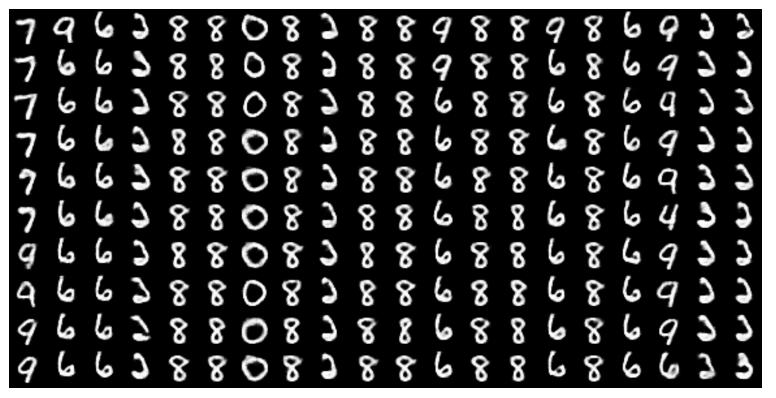
\includegraphics[scale=0.4]{img/rbm_samples.png}
\centering
\caption{Samples generated by the RBM after PCD-15 training on MNIST. Each row represents a mini-batch of negative particles (samples from independent Gibbs chains). 1000 steps of Gibbs sampling were taken between each of those rows.}
\label{fig:rbm_samples}
\end{mdframed}
\end{figure}

\subsubsection{Visual Inspection of Filters}
The filters learnt by the model can be visualized. This amounts to plotting the weights of each unit as a gray-scale image (after reshaping to a square matrix). Filters should pick out strong features in the data. While it is not clear for an arbitrary dataset, what these features should look like, training on MNIST usually results in filters which act as stroke detectors, while training on natural images lead to Gabor like filters if trained in conjunction with a \tb{sparsity criteria} (more details in next subsections). For example, see Fig. \ref{fig:rbm_filters}. It is worth noting that filters may or may not be \emph{sparse}. If filters are sparse, they will respond to very local features. Dense filters, on the other hand, respond to stimuli across the entire filter. Although the two types
of filter are qualitatively different, in \cite{yosinski2012visually} they observed cases in which both types are successful in learning the underlying density.
\begin{figure}[h]
\begin{mdframed}
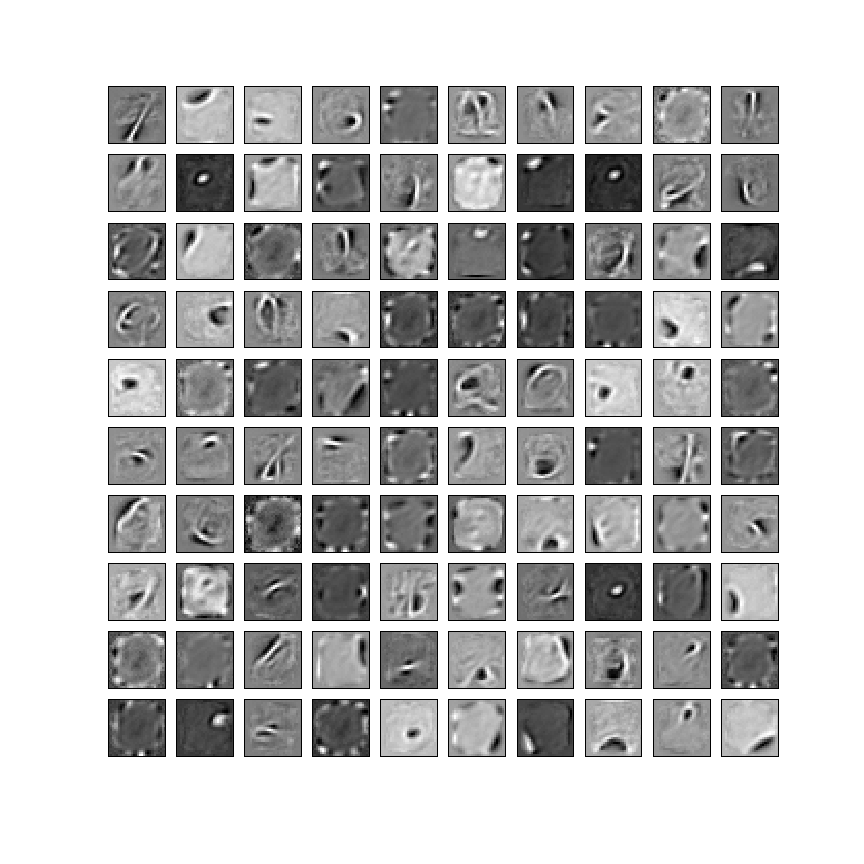
\includegraphics[scale=0.4]{rbm-mnist/rbm_filters.png}
\centering
\caption{Filters learned by RBM after CD-1 training on MNIST.}
\label{fig:rbm_filters}
\end{mdframed}
\end{figure}

\subsubsection{Probabilities of hidden activations}
It is useful to plot activations of hidden neurons to see how they are being used, how often they are likely to be on vs. off, are there any "dead" neurons (which are always on of always off) etc. This can be effectively done by plotting greyscale matrix of probabilities of (some) hidden units for each of the input example in a minibatch, for instance. For example, see Fig. \ref{fig:rbm_hidden_activations}.
\begin{figure}[h]
\begin{mdframed}
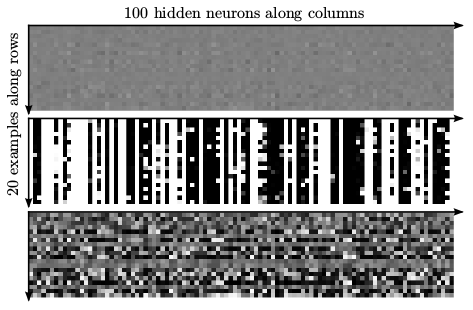
\includegraphics[scale=0.64]{img/rbm_hidden_activations.png}
\centering
\caption{Hidden neuron activation probabilities for the first 100 neurons (of 1,000) and the first 20 example data points (of 50,000), where black represents p = 0 and white, p = 1. Each row shows different neurons’ activations for a given input example, and each column shows a given neuron’s activations across many examples. Top: correct dithered gray before training begins. Values are mostly in [.4, .6]. Middle: Values pegged to black or white after one mini-batch. Decrease initial $\mb{W}$ values or learning rate. Bottom: the learning has converged well after 45 epochs of
training.}
\label{fig:rbm_hidden_activations}
\end{mdframed}
\end{figure}
\\[1em]Before any training, the probability plot should be mostly a flat gray, perhaps with a little visible noise. That is, most hidden probabilities should be around .5, with some as low as .4 or as high as .6. If the plot is all black (near 0) or all white (near 1), the weights or hidden biases were set incorrectly. The weights $\mb{W}$ should initially be random and centered at 0, and hidden biases should be zero or at least centered at zero. If the probability plot contains both pixels pegged to black and pixels pegged to white, then the $\mb{W}$ has been initialized with values too large. Intuitively, the problem with this case is that all hidden neurons have already determined what features they are looking for before seeing any of the data. 
\\
\tb{TL;DR:} when learning is working properly, this display should look thoroughly random w/o any obvious vertical or horizontal lines.

\subsubsection{Distribution/histograms of weights and weights updates}
In addition to the hidden probability plots above, it is often useful to monitor distributions of the model parameters (weights and biases) themselves, and their corresponding parameters \tb{updates} (for vanilla SGA (stoch. gradient ascent) they are gradient$\times$learning rate, and slightly more complicated formulae when using momentum or others more advanced variants of SGA). Under normal, desired conditions in the middle of
training, all histograms should look roughly Gaussian in shape, and the mean magnitudes of parameters updates should be smaller by a factor of $10^2$ to $10^4$ than mean magnitudes of the respective parameters. If the change in weights is too small (i.e. a separation of more than
$10^4$), then the learning rate can probably be increased. If the change in weights is too large, the learning may explode and the weights diverge to infinity.

\subsubsection{Proxies to Likelihood}
Other, more tractable functions can be used as a proxy to the likelihood. When training an RBM with CD/PCD, one can use \tb{pseudo-likelihood} as the proxy. Pseudo-likelihood (PL) is much less expensive to compute, as it assumes that all bits are independent
\bg
\text{PL}(\mb{v})=\prod_{i=1}^D p(v_i|\mb{v}_{-i}), \text{ and}
\\
\text{PLL}(\mb{v}):=\log \text{PL}(\mb{v})=\sum_{i=1}^D \log p(v_i|\mb{v}_{-i})
\eg
[  Compare to $\log p(\mb{v})=\log p(v_1)+\log p(v_2|v_1) +\ldots + \log p(v_D|\mb{v}_{1:D-1})$  ].
\\[1em]
For general probabilistic graphical model, $\log p(v_i|\mb{v}_{-i})=\log p(v_i|\mb{v}_{\mc{N}(i)})$, where $\mc{N}(i)$ -- set of neighbors of variable $i$. One can show that estimation by maximizing the pseudolikelihood is asymptotically consistent \cite{goodfellow2016deep}.
\\[1em]
\u{Lets calculate $p(v_i=1|\mb{v}_{-i})$ for RBM} (omit $\bs{\psi}$ for brevity)
\begin{empheq}[box={\mybox[1em][1em]}]{gather*}
p(v_i=1|\mb{v}_{-i})=\frac{p(v_i=1,\mb{v}_{-i})}{p(\mb{v}_{-i})}=\frac{p(v_i=1,\mb{v}_{-i})}{p(v_i=1,\mb{v}_{-i})+p(v_i=0,\mb{v}_{-i})}=
\frac{\frac{1}{Z}e^{-\mc{F}(v_i=1,\mb{v}_{-i})}}{\frac{1}{Z}e^{-\mc{F}(v_i=1,\mb{v}_{-i})} + \frac{1}{Z}e^{-\mc{F}(v_i=0,\mb{v}_{-i})}}=
\\=\frac{e^{-\mc{F}(v_i=1,\mb{v}_{-i})}}{e^{-\mc{F}(v_i=1,\mb{v}_{-i})} + e^{-\mc{F}(v_i=0,\mb{v}_{-i})}}=\frac{1}{1 + e^{-\l[\mc{F}(v_i=0,\mb{v}_{-i})-\mc{F}(v_i=1,\mb{v}_{-i})\r]}}=\text{sigm}\l[\mc{F}(v_i=0,\mb{v}_{-i})-\mc{F}(v_i=1,\mb{v}_{-i})\r]
\end{empheq}
So:
\begin{gather}
\boxed{p(v_i=1|\mb{v}_{-i})=\text{sigm}\l[\mc{F}(v_i=0,\mb{v}_{-i})-\mc{F}(v_i=1,\mb{v}_{-i}) \r)}
\end{gather}
Note how this formula (and derivation) resembles formulae (11),(12). This is because free energy is designed as $p(\mb{v})\;\propto \;e^{-\mc{F}(\mb{v})}=:p^*(\mb{v})$, similarly to $p(\mb{v},\mb{h})\;\propto \;e^{-E(\mb{v},\mb{h})}=:p^*(\mb{v},\mb{h})$. We also reduced complexity to only $O(V)$ invocations of unnormalized probability $p^*(\mb{v})$ instead of $O(2^{V+H})$ invocations of $p^*(\mb{v},\mb{h})$ to compute partition function for true log-likelihood.
Using equations (49),(50),(43), we can now compute PLL, which is the sum of the log-probabilities of each bit/feature $v_i$, conditioned on the state of all other bits. For moderate $D$ (e.g. for MNIST $D=784$), this sum remains rather expensive. For this reason, the following stochastic approximation to PLL is often used \cite{tutorial2014lisa, scikit-learn}:
\bg
\boxed{  \t{\text{PLL}}(\mb{v})=D\cdot \log \text{sigm}\l( \mc{F}(\t{\mb{v}}_{\tau})-\mc{F}(\mb{v}) \r), \;\;\tau \sim U(\{1\ldots D\})  },
\eg
where $\t{\mb{v}}_{i}$ is $\mb{v}$ with $i$-th bit flipped (0 $\rightarrow$ 1, 1 $\rightarrow$ 0).\\
\tb{Note}: $\E_{\tau}[\t{\text{PLL}}(\mb{v})]=\text{PLL}(\mb{v})$.
\\
\tb{Note}: Do not compute $\log \text{sigm}(x)$ naively, it is numerically unstable operation. Either observe that $\log \text{sigm}(x)=-\text{softplus}(-x)$ and use numerically stable implementation of softplus or use built-in functions (e.g. \texttt{tf.log\_logistic} in TensorFlow $\geq$ 1.2).
\\[1em]
This stochastic approximation uses only $2=O(1)$ invocations of $p^*(\mb{v})$/free-energy \tb{per training example}. Note that typically one compute average free-energy over all (or subset of) training set.
\\[1em]
\tb{Note} Some also monitor \emph{reconstruction error} during training. Although it is convenient, it is poor measure of actual RBM performance, since this is not the function Contrastive Divergence optimizes. However, typically, nicely trained model has low reconstruction error.
\\[1em]
Also there is Markov-chain based method to estimate partition function of RBM called \emph{Annealed Importance Sampling} \cite{salakhutdinov2013learning}, which can be used to estimate log-probabilities of validation data directly. We will use this methods for DBMs.

\subsubsection{Monitoring overfitting: Free energy gap}
Unfortunately, for large RBMs, it is very difficult to compute this probability
because it requires knowledge of the partition function. Nevertheless, it is possible to directly monitor
the overfitting by comparing the free energies of training data and held out validation data. In this
comparison, the partition function cancels out. As we saw, the free energy of a data vector can be computed in
a time that is linear in the number of hidden units. As the
model starts to overfit the average free energy of the validation data will rise relative to the average
free energy of the training data and this \emph{gap} represents the amount of overfitting. (Since $p(\mb{v})\propto e^{-\mc{F}(\mb{v})}$ this means network will put noticeably higher probability to training data). Free energy can be computed for subset of training (and validation data), but the same subsets should be used for the whole training.

\subsection{Choice of hyperparameters, various tricks to improve/speedup learning}
Most of the tricks and recipes are taken from \cite{hinton2010practical}.

\subsubsection{Number of Gibbs steps}
In theory the more steps we use to estimate model expectations, the better approximation of gradients we should obtain, and better learning should be observed.
\\[0.5em]
\bad However, in my experiments on MNIST, more steps decrease performance for both RBM and DBM in terms of both pseudo-loglik and quality of filters and samples.
\\
\textbullet{} In \cite{hinton2010practical} they suggest to gradually increase $k$ in CD-k during training. This is not currently implemented.

\subsubsection{Updating hidden and visible states}
The question can we or should we use probabilities instead of samples in update rules of contrastive divergence (31)-(33). It is very important to make hidden units driven by data stochastic -- this will act as a strong regularizer (network won't be able to communicate real values to the hidden units -- information bottleneck). Further updates of hidden units and all updates of visible units should use probabilities instead of sampling for less noisy and faster learning.
\\[0.5em]
\bad In the experiments if data-driven hidden units were sampled and for the rest probabilities were used, this model had the lowest pseudo-likelihood and sharp filters, see Fig. \ref{fig:rbm_sampling}. This is typically means overfitting
\\
\textbullet{} If probabilities were used only for visible units, this model had the highest PLL, but still some of the filters were sharp. This model is best suited for supervised tasks (e.g. finetuning using backprop for classification)
\\
\textbullet{} If both hidden and visible units are sampled when estimating model statistics, the learned filters are smooth and large number of them are sparse. This model has slightly worse PLL, thus we observe underfitting. When RBMs are trained to learn compound models, such as DBMs/DBNs, generative model is not the ultimate objective and it may be possible to save time by underfitting it.
\\
\good Data-driven hidden states should absolutely be sampled.
\begin{figure}[h]
\begin{mdframed}
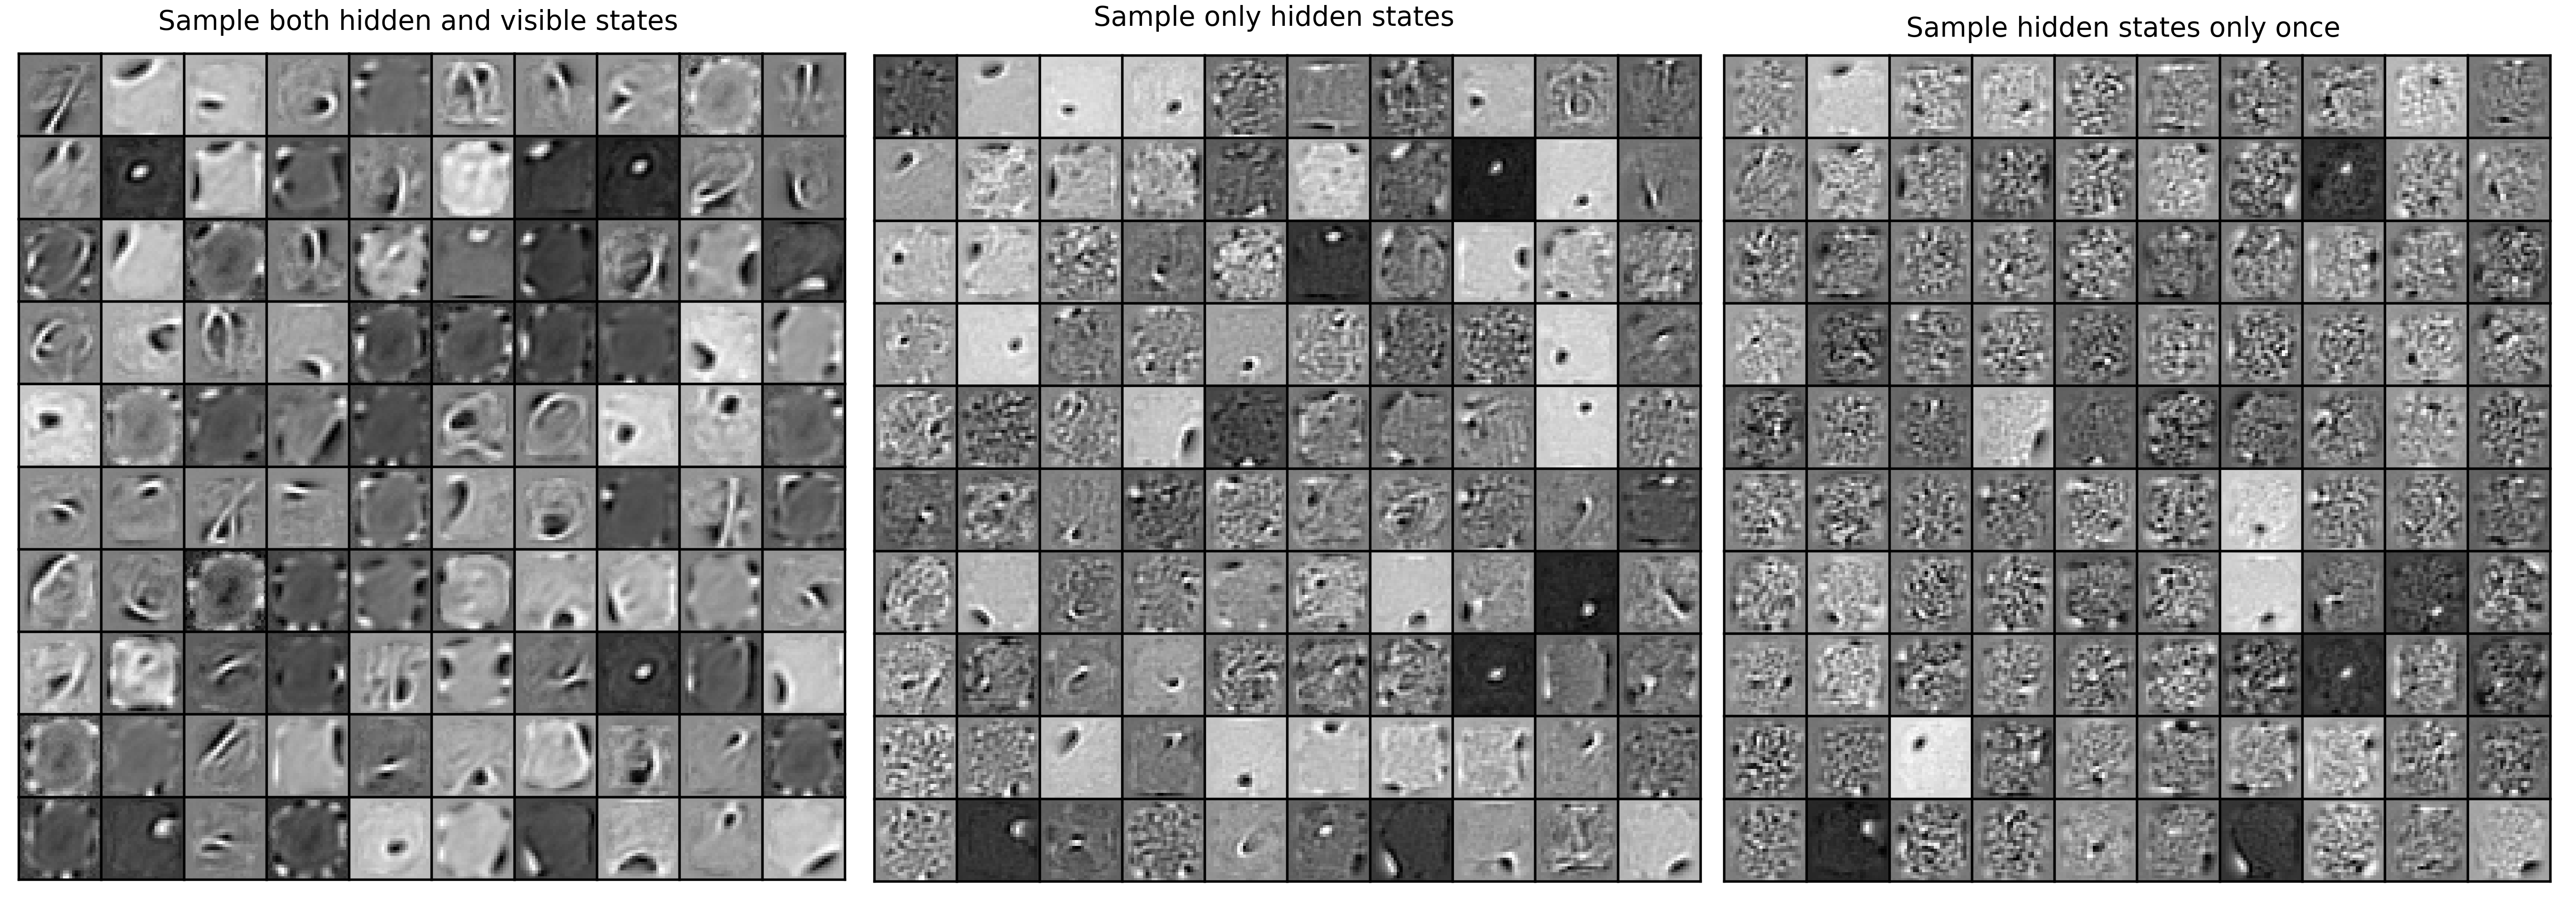
\includegraphics[scale=0.17]{rbm-mnist/rbm_sampling.png}
\centering
\caption{RBM filters trained on MNIST depending on whether to sample hidden and/or visible units.}
\label{fig:rbm_sampling}
\end{mdframed}
\end{figure}

\subsubsection{Minibatch size}
\good It is a serious mistake to make batchsizes too large. Batch size of 1 is ok, but more efficient 10-100 for more efficient computations using linalg libraries. For datasets that contain a small number of equiprobable classes, the ideal mini-batch size is often
equal to the number of classes and each mini-batch should contain one example of each class.

\subsubsection{Learning rate}
\good Shouldn't be too high (weights could explode) and not too low (slow learning). Typically it should be from $10^{-4}$ to $10^{-2}$ of order of magnitude of weights (check histogram).
\\
\good For Gaussian visible units the learning rate needs to be about one or two orders of magnitude smaller than when using binary visible units.
\\
\textbullet{} For larger $k$ in CD-k and in case of Persistent CD-k it is reasonable to slightly reduce learning rate.

\subsubsection{Initial values of the weights and biases}
\good weights are typically initialized to small zero-centered Gaussian random variables with std of about 0.01 (too large could speedup learning but also can cause "died" units (with either too large or too small activation probabilities), which slows learning).
\\
\textbullet{} weights can also be initialized to zeros, but only if hidden states are sampled (this way they still will be different even if they initially had identical connectivities)
\\
\good it is usually helpful to initialize the bias of visible unit $i$ to $\log[p_i/(1-p_i)]=\text{sigm}^{-1}(p_i)$, where $p_i$ is the proportion of training vectors in which unit $i$ is on. This will ensure that in early stages of training visible units will have activation probabilities close to $p_i$. Models with such initialization had noticeably higher PLL on MNIST.
\\
\textbullet{} $\log[t/(1-t)]=\text{sigm}^{-1}(t)$ for hidden units if sparsity target $t$ is used, otherwise zero.
\\
\bad Do not initialize hidden biases to large negative values, like $-4$ to crudely encourage sparsity. Such models had lower PLL and worse filters.

\subsubsection{Momentum method}
\good Using momentum dramatically speedups learning. In \cite{hinton2010practical} and \cite{dbm_code} they suggest to start with 0.5 and after couple of epochs to instantly increase momentum to 0.9. I found that gradually increasing momentum from 0.5 to 0.9 is slightly better. Common constant schedules for momentum, like 0.9 are also fine.

\subsubsection{Weight decay}
\good It definitely helps, and there are multiple reasons to use weight decay (not only to prevent overfitting!):
\begin{itemize}
	\item to improve generalization by preventing overfitting
	\item "unstick" hidden units that were either firmly "on" or "off"
	\item improve mixing rate of Gibbs chain which makes CD better approximate log-likelihood gradients etc.
\end{itemize}
Good values for weight decay coefficient are $10^{-5}\ldots10^{-2}$.

\subsubsection{Different regularization techniques}
\textbullet{} L1 weight-decay often leads to strongly localized receptive fields (many of the weights to become exactly zero whilst allowing a few of the weights to grow quite large, this can make it easier to interpret the weights).
\\
\textbullet{} Maxnorm helps to avoid hidden units getting stuck with extremely small weights, but a sparsity target is probably a better way to avoid this problem. Maxnorm will play more important role in DBM training, though.
\\
\textbullet{} Dropout: does not seem to help in any way.  

\subsubsection{Encouraging sparse hidden activities: sparsity targets}
Sparse activities of the binary hidden units can be achieved by specifying a "sparsity target" which is the desired probability of being active, $t<<1$ (typically $t=0.01$ to $t=0.1$. An additional penalty term is then used to encourage the actual probability of being active $q$ to be close to $t$. $q$ is estimated by using an exponentially decaying average of the mean probability that a unit is active in each mini-batch:
\bg
q \leftarrow \omega q + (1-\omega) q_{\text{current}},
\eg
where $q_{\text{current}}$ is the mean activation probability of the hidden unit on the current mini-batch, decay rate $\omega$ is typically 0.9 to 0.99. For logistic hidden units the natural penalty measure to use is the cross entropy between the desired and actual distributions:
\bg
\text{Sparsity penalty}=\lambda\times\l[ -t\log q-(1-t)\log(1-q) \r],
\eg
where $\lambda$ is a hyperparameter called "sparsity cost". (53) has simple derivative of $\lambda (q-t)$ w.r.t. total input of a unit. It is imprtant to apply the same derivative to both weights and hidden biases. Histogram the mean activities of the hidden units and set the sparsity-cost so that the hidden units have mean probabilities in the vicinity of the target. If the probabilities are tightly clustered around the target value, reduce the sparsity-cost so that it interferes less with the main objective of the learning.

\subsubsection{Number of hidden units}
\good It is common and useful to use more hidden units than visible, especially in conjunction with a sparsity target. (In discriminative learning labels usually contain very few bits of information, so using more parameters than training cases will typically cause severe overfitting; when learning generative models of high-dimensional data, however, it is the number of bits that it takes to specify a data vector that determines how much constraint each training case imposes on the parameters of the model. This can be several orders of magnitude greater than number of bits required to specify a label.)

\subsection{Experiments}
Also check jupyter notebooks in github repo. All RBMs here are trained on MNIST.

\begin{figure*}[t!]
\begin{mdframed}
\centering
\begin{subfigure}[t]{0.5\textwidth}
    \centering
    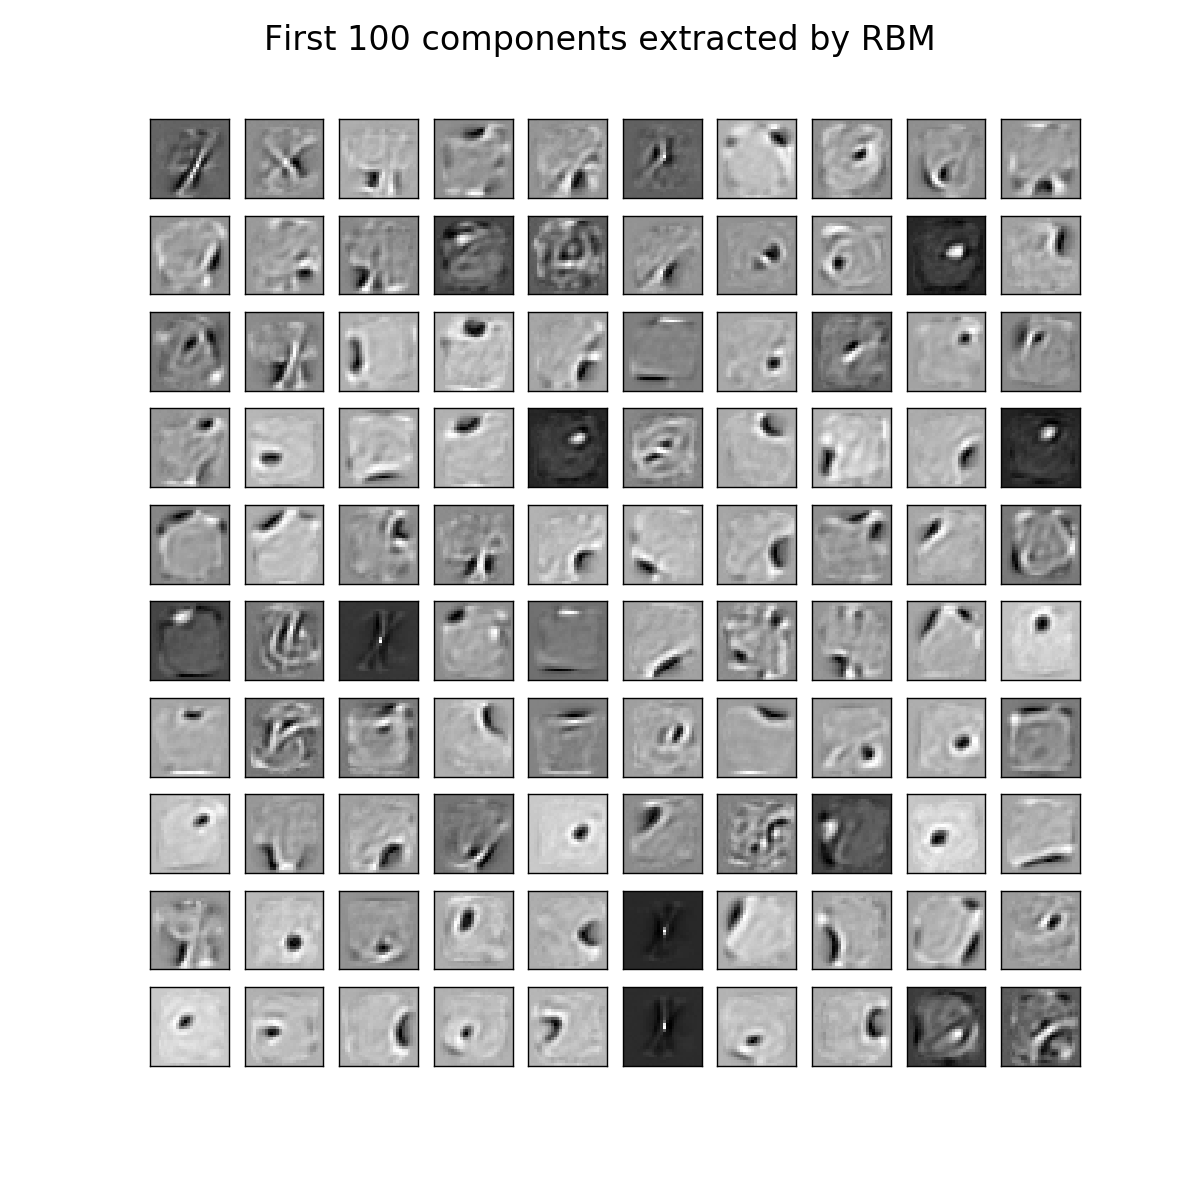
\includegraphics[height=3.2in]{rbm-mnist/rbm_mnist_256.png}
    \caption{256 hidden layers}
\end{subfigure}%
~
\begin{subfigure}[t]{0.5\textwidth}
    \centering
    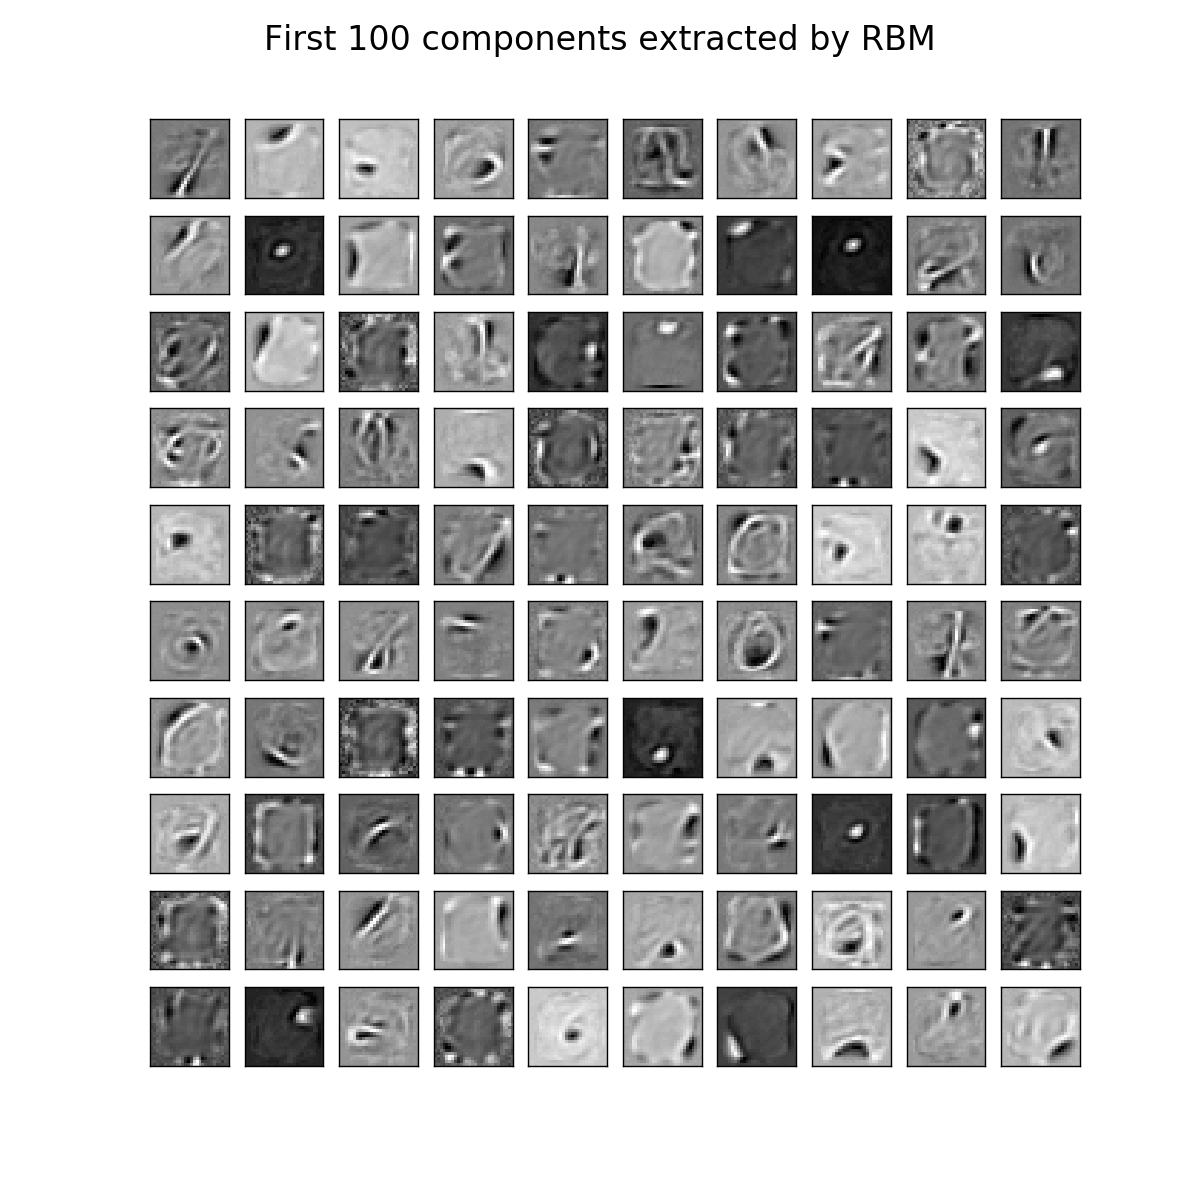
\includegraphics[height=3.2in]{rbm-mnist/rbm_mnist_1024.png}
    \caption{1024 hidden layers}
\end{subfigure}
\caption{Different number of hidden layers}
\end{mdframed}
\end{figure*}

\begin{figure}[h]
\begin{mdframed}
\centering
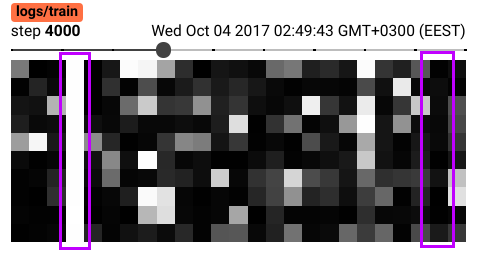
\includegraphics[width=4.2in]{rbm-mnist/dropout.png}
\caption{Dropout $p=0.9$ kills some hidden units.}
\end{mdframed}
\end{figure}

\clearpage

\begin{figure}[h]
\begin{mdframed}
\centering
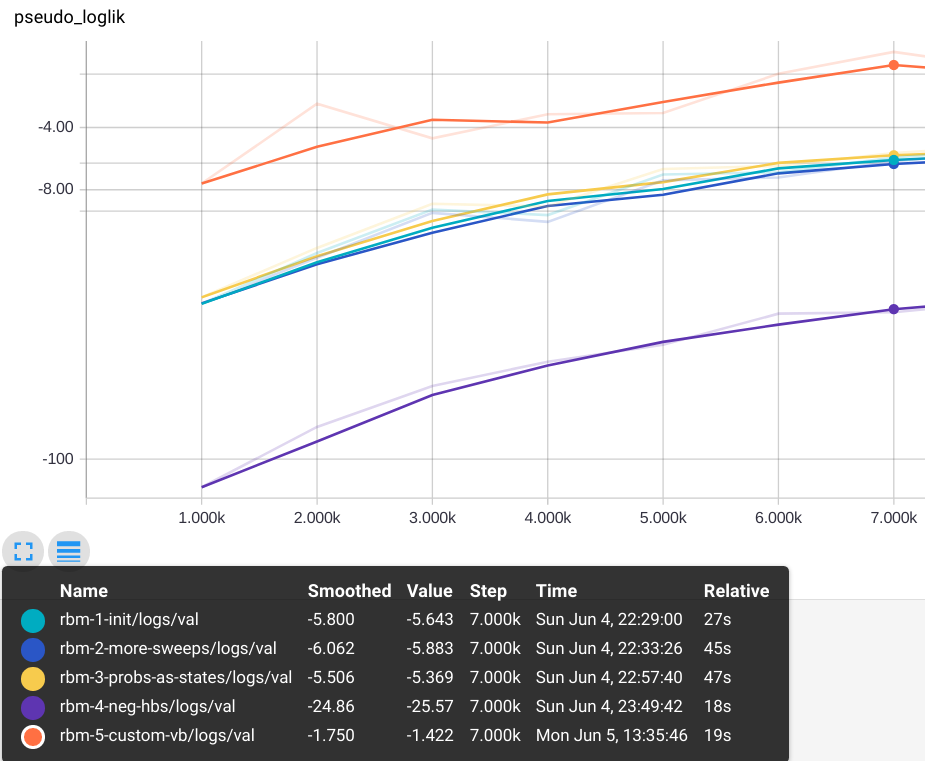
\includegraphics[width=4.8in]{rbm-mnist/rbm-runs_10k.png}
\\[2em]
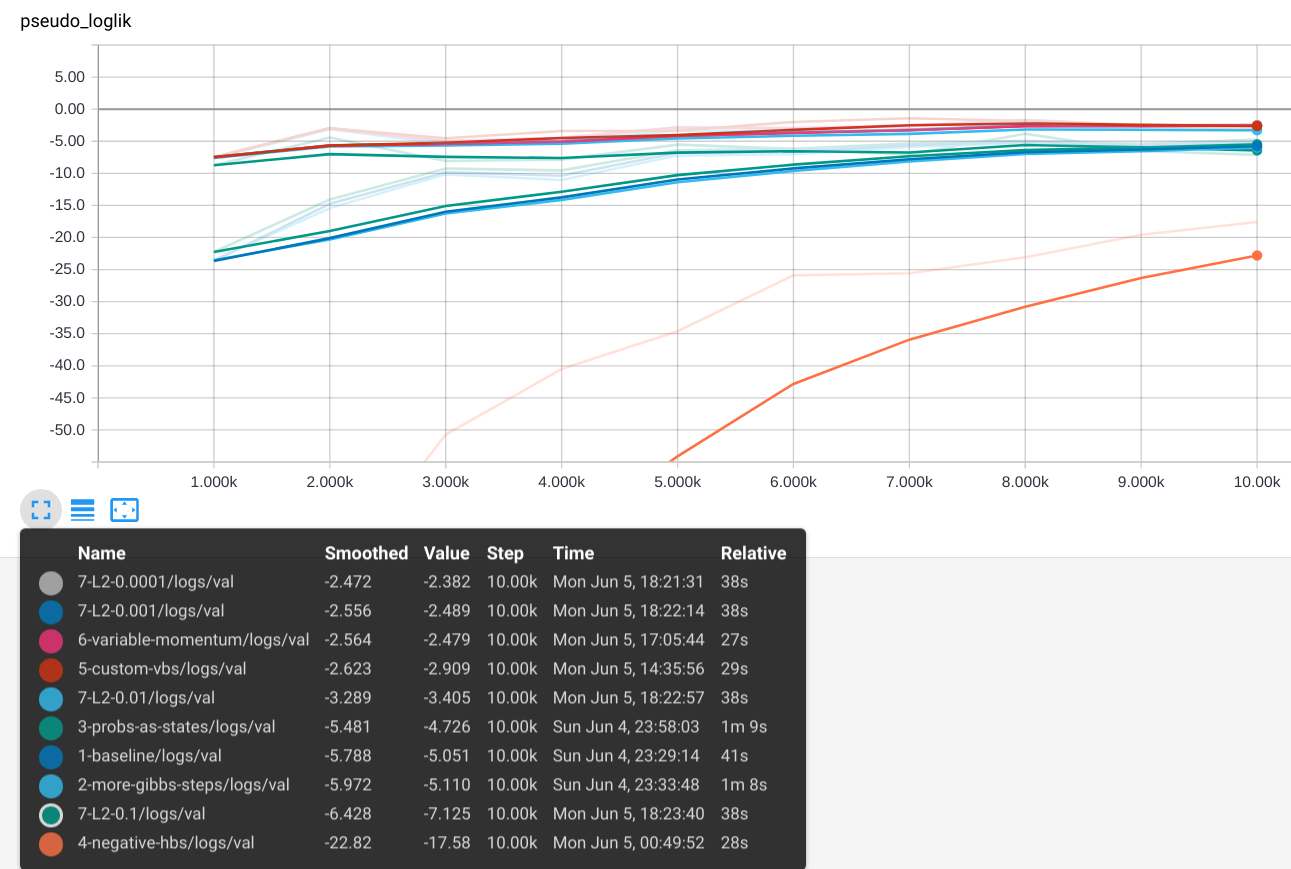
\includegraphics[width=4.8in]{rbm-mnist/rbm_practical_10k.png}
\caption{PLL of RBMs trained using various approaches on 10k MNIST digits.}
\end{mdframed}
\end{figure}

\clearpage

\begin{figure*}[t!]
\begin{mdframed}
\centering
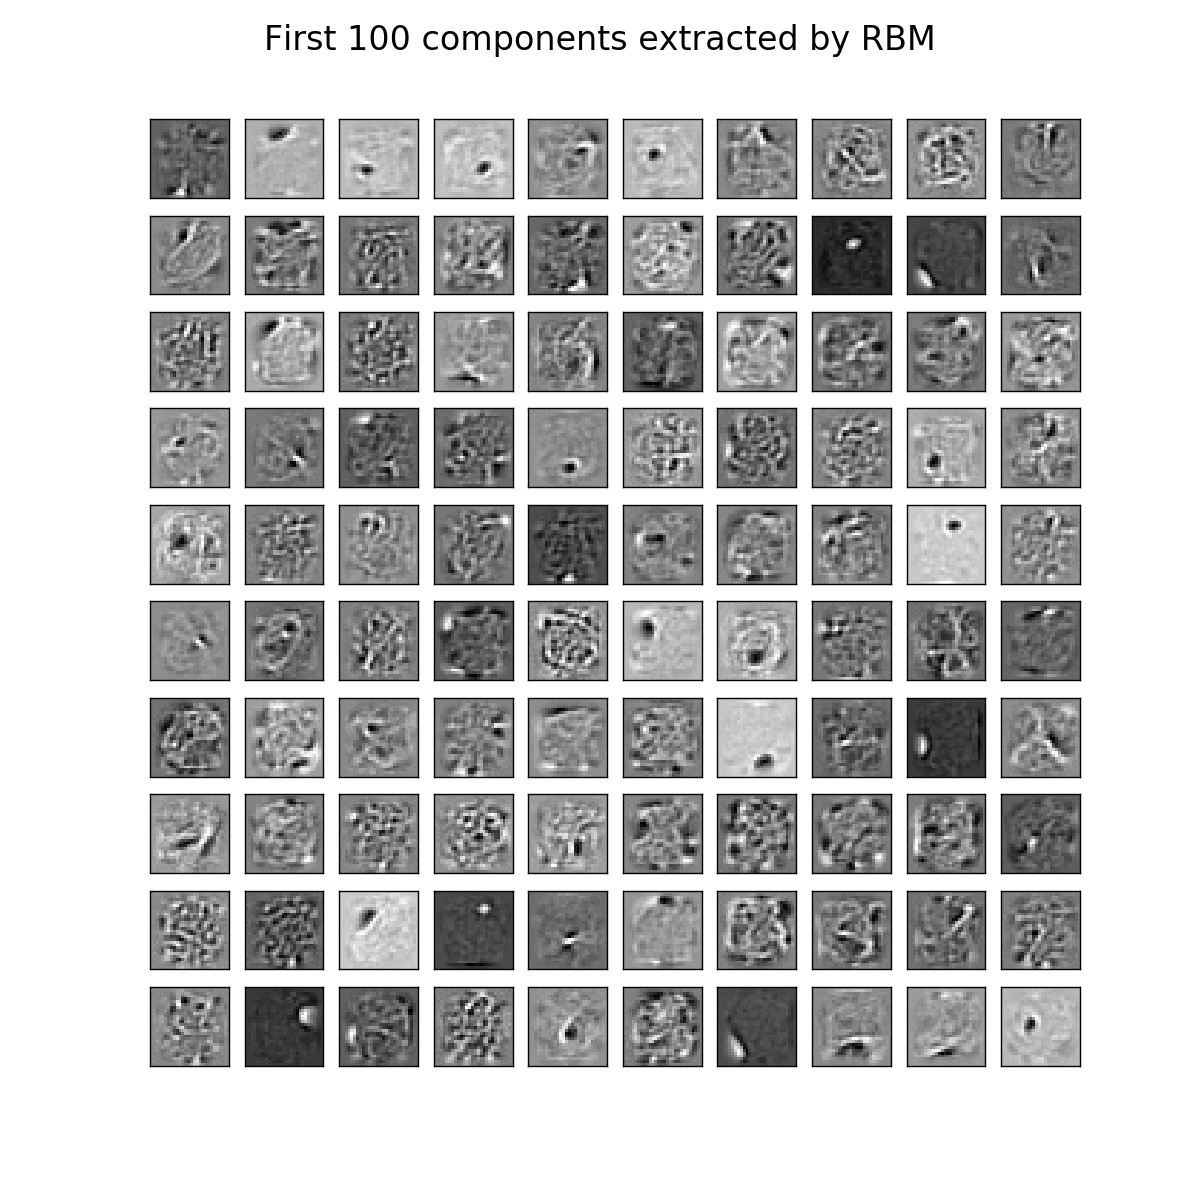
\includegraphics[width=.31\textwidth]{rbm-mnist/L1e-5.png}\quad
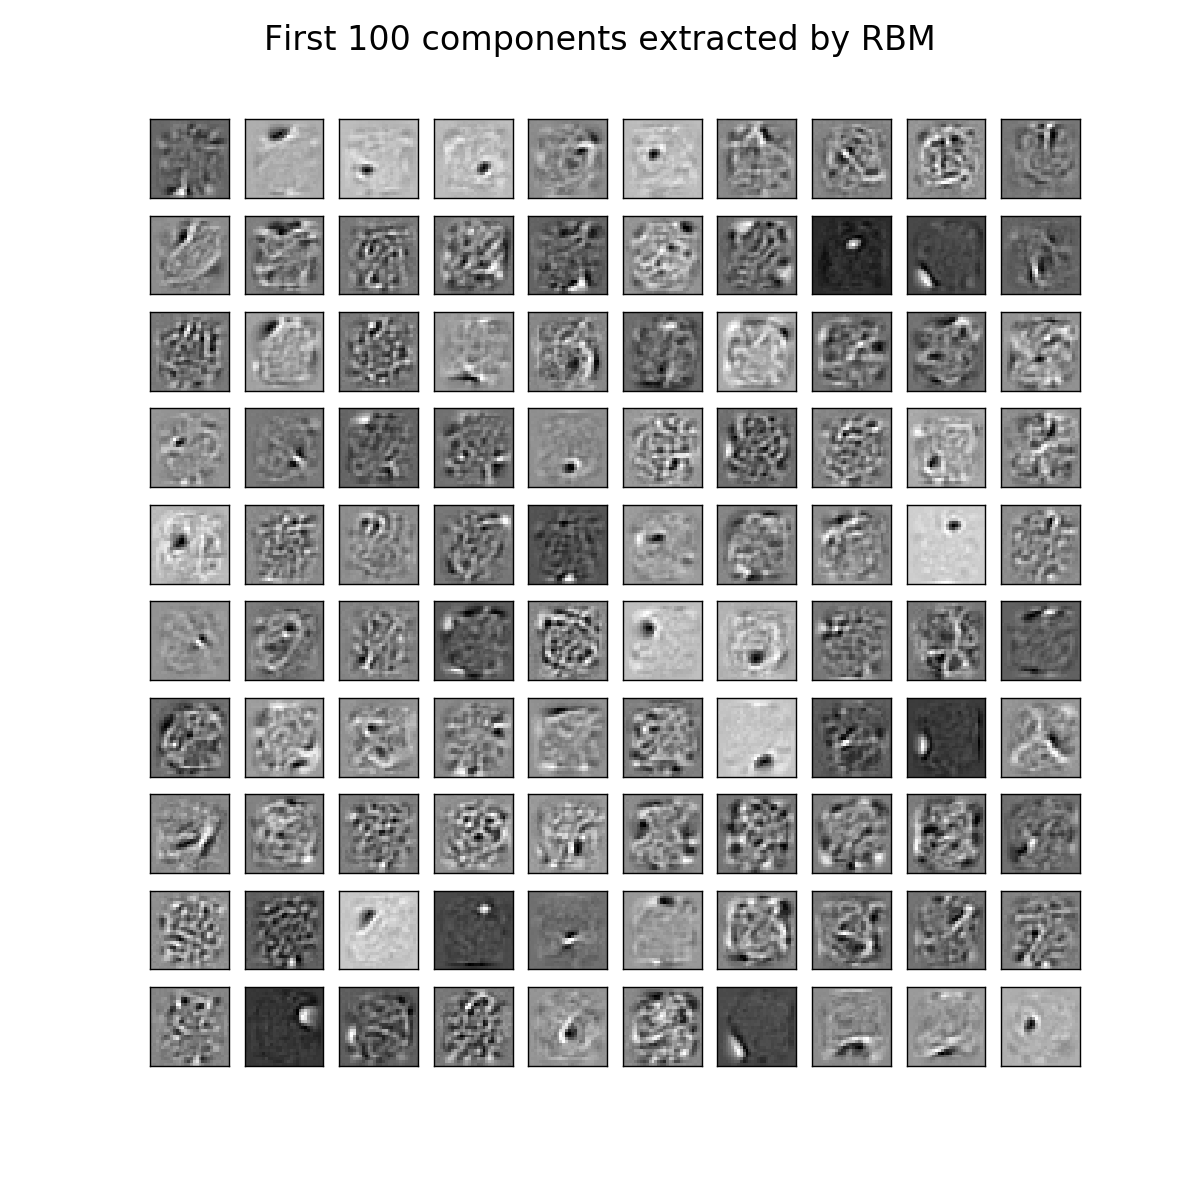
\includegraphics[width=.31\textwidth]{rbm-mnist/L1e-4.png}\quad
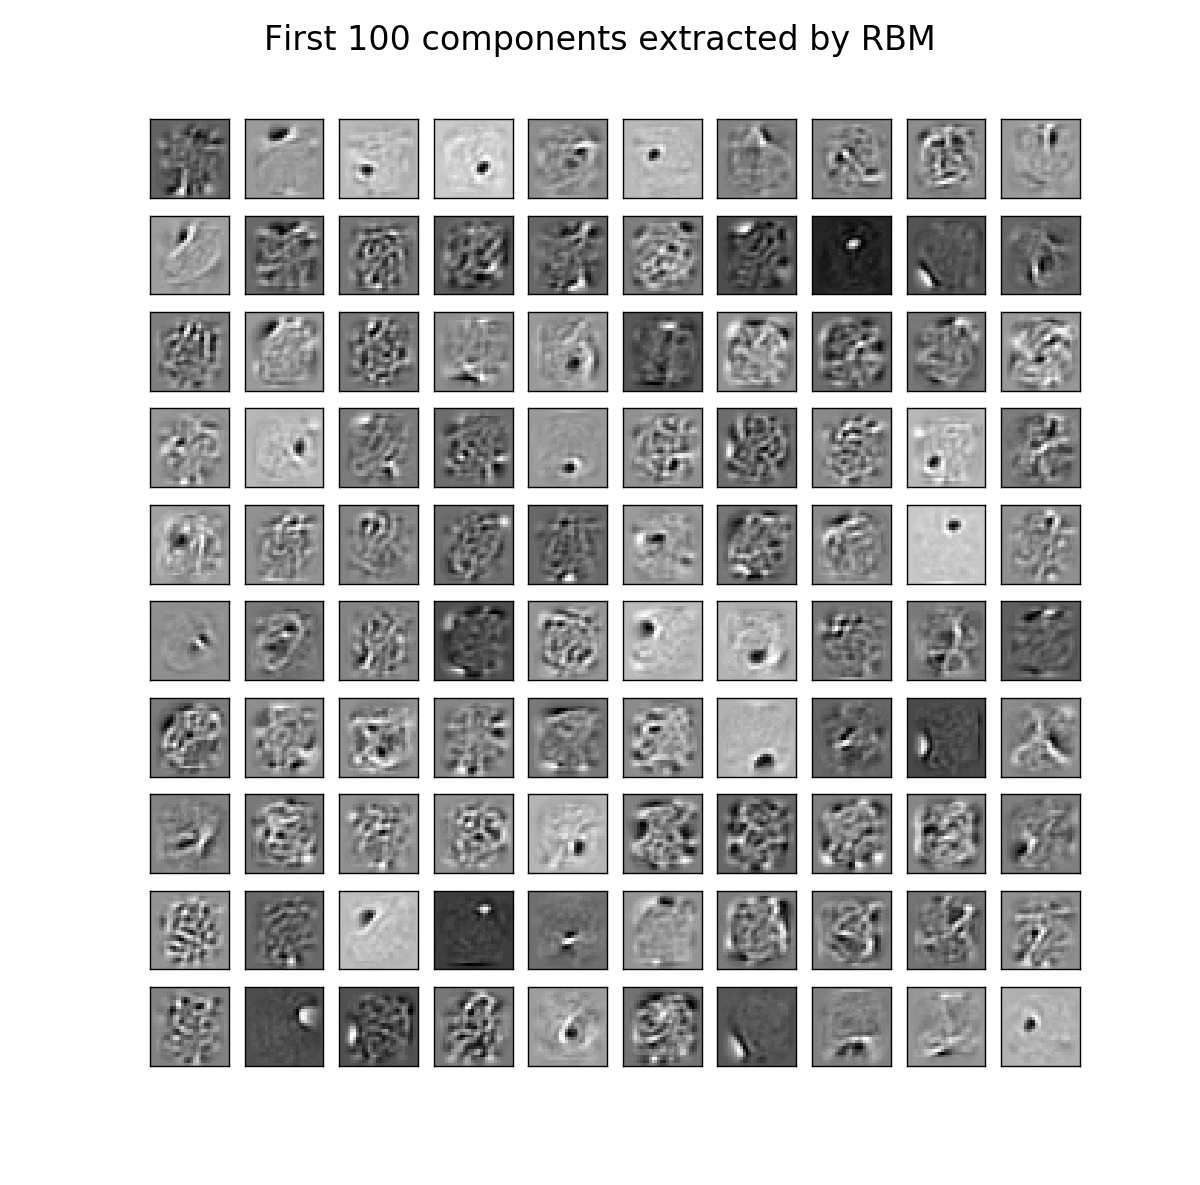
\includegraphics[width=.31\textwidth]{rbm-mnist/L1e-3.png}

\medskip

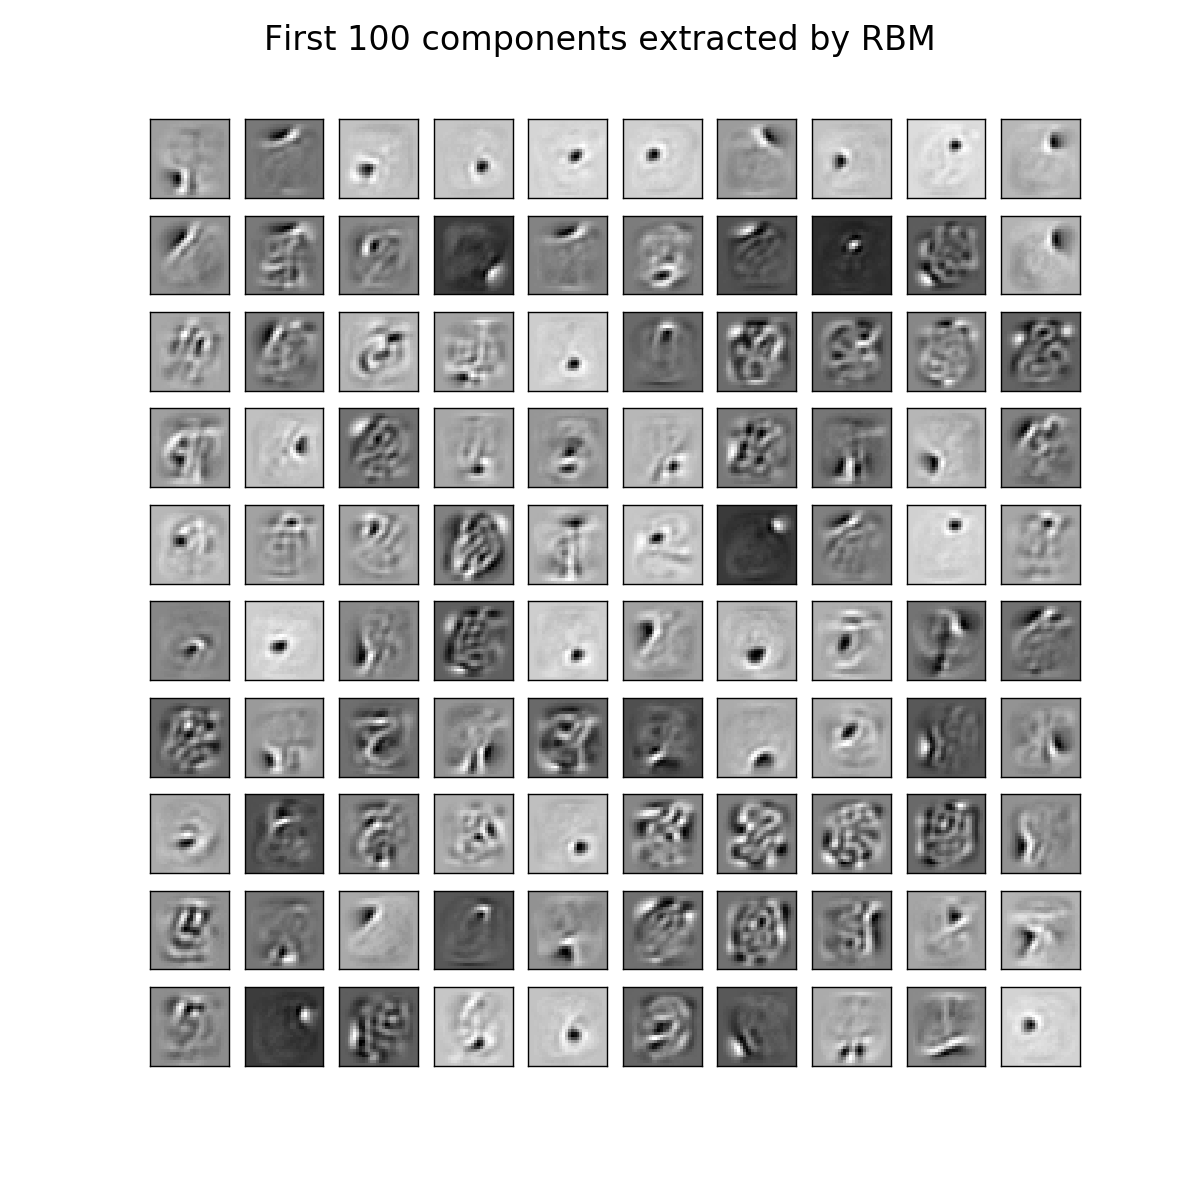
\includegraphics[width=.32\textwidth]{rbm-mnist/L1e-2.png}\quad
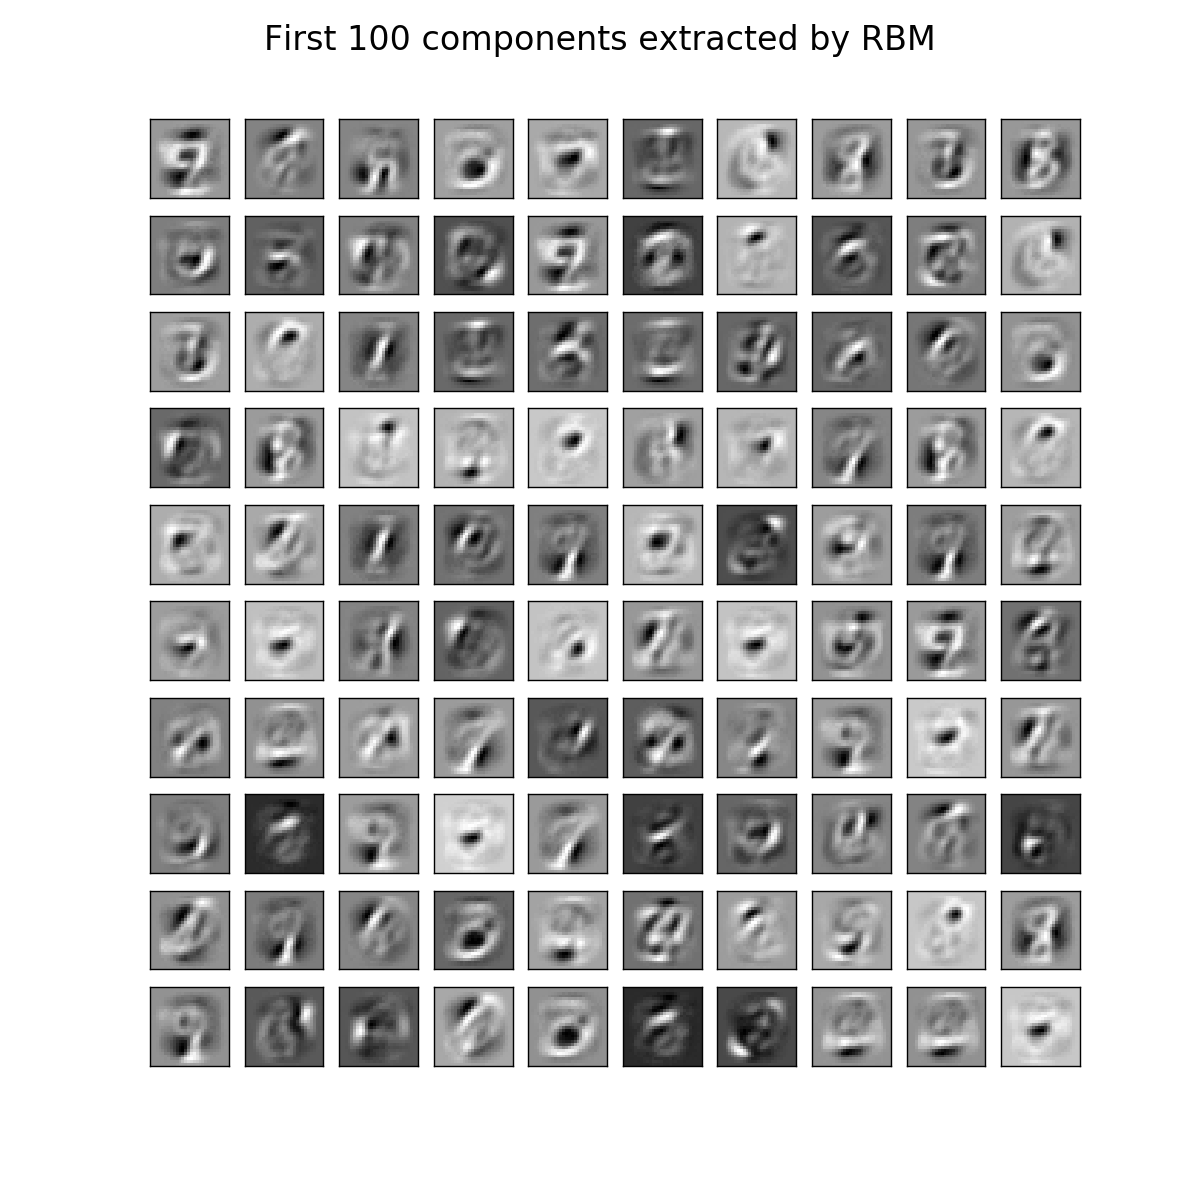
\includegraphics[width=.32\textwidth]{rbm-mnist/L1e-1.png}

\medskip

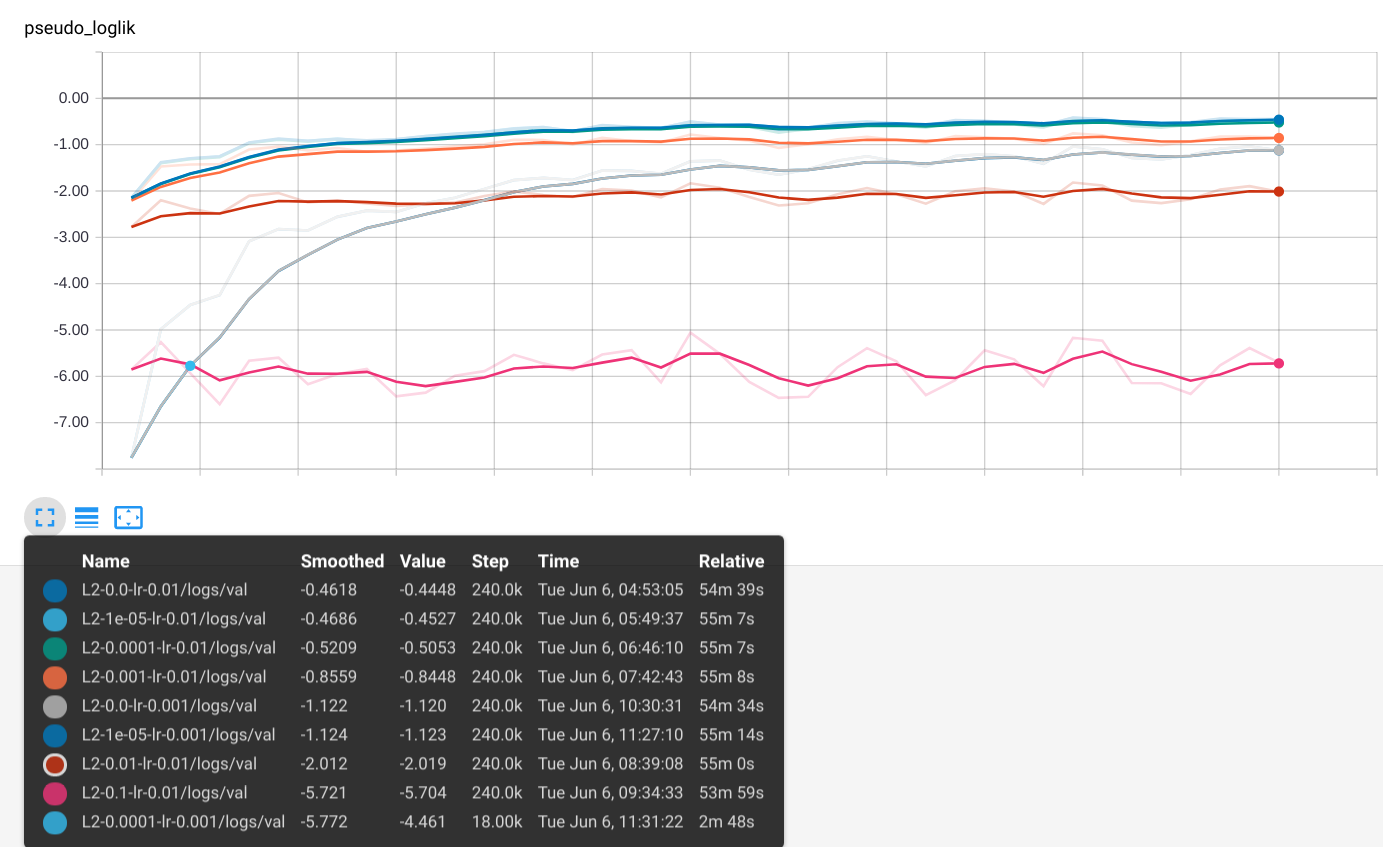
\includegraphics[width=.9\textwidth]{rbm-mnist/L2_pll.png}
\caption{Different amount of regularization. \emph{Left to right, top to bottom}, $\lambda=10^{-5}\ldots10^{-1}$. \emph{Bottom}: PLL of RBM as $\lambda$ varies.}
\end{mdframed}
\end{figure*}

\clearpage

\begin{figure}[h]
\begin{mdframed}
\centering
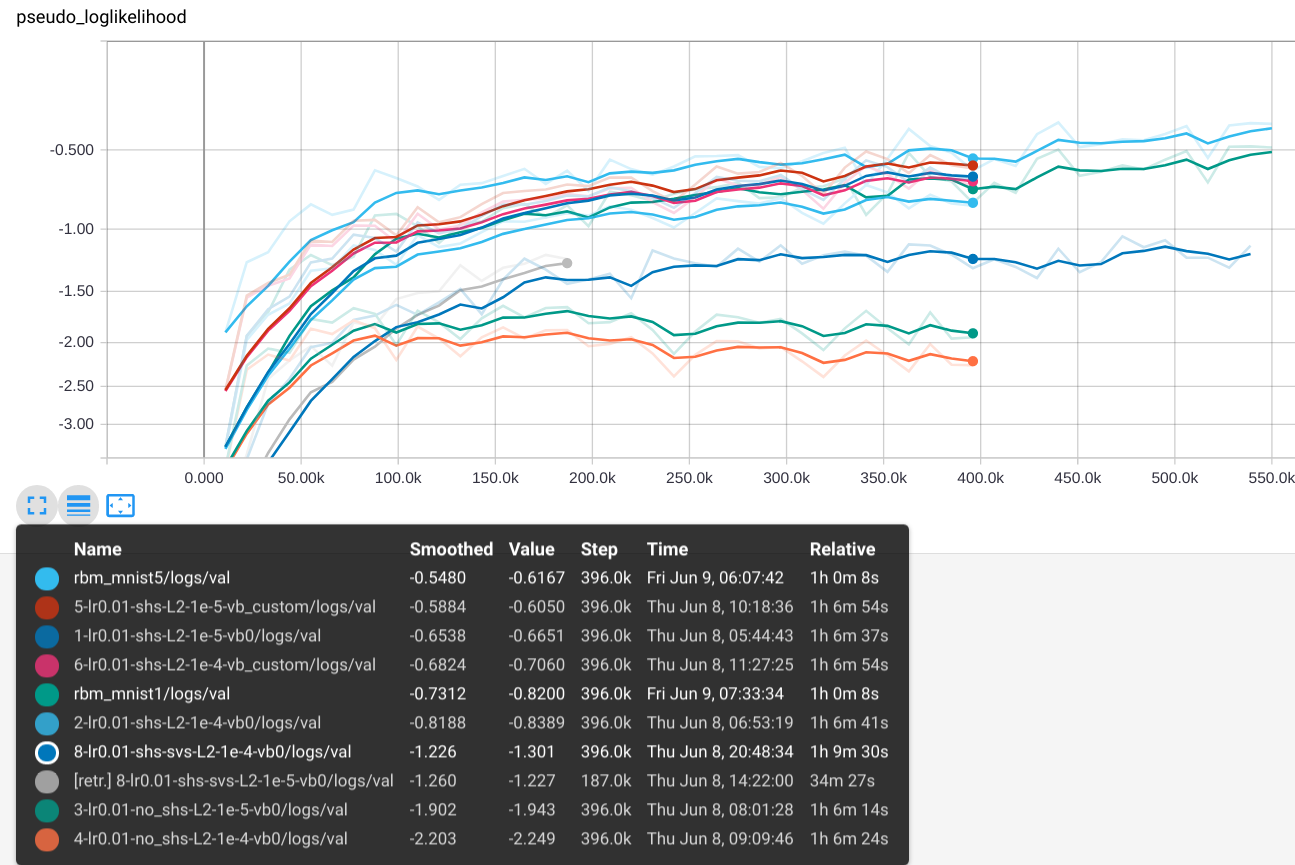
\includegraphics[width=4.6in]{rbm-mnist/rbm_practical_full.png}
\\[1em]
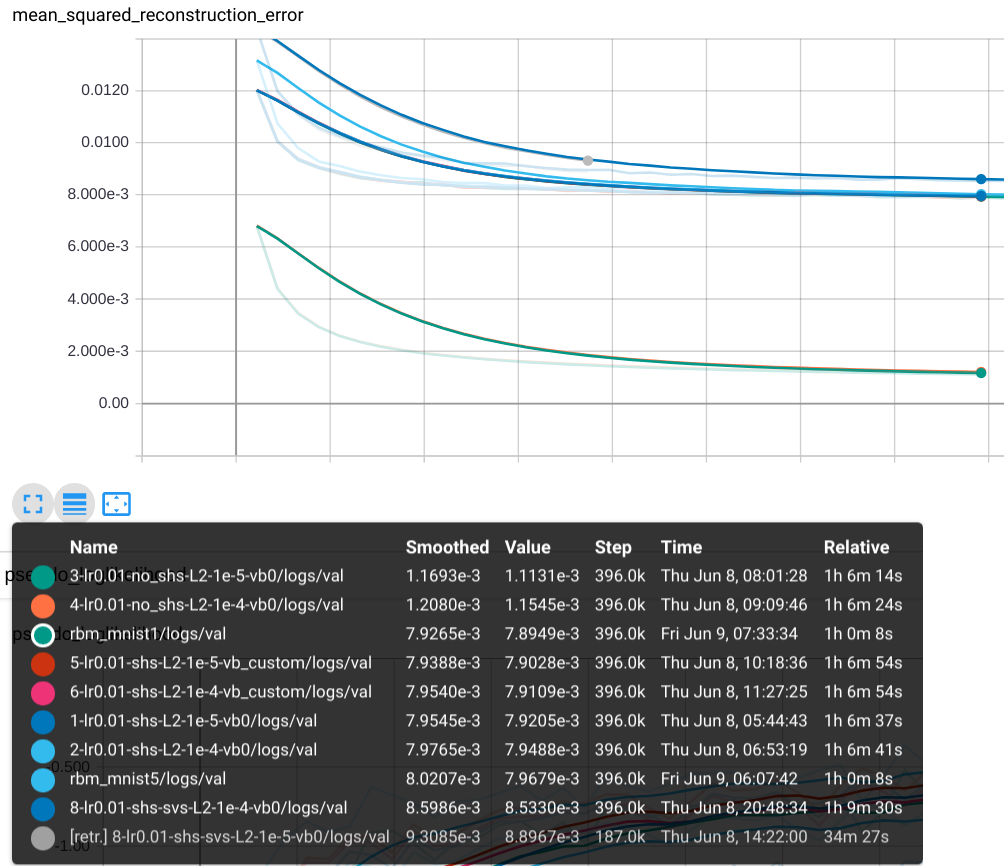
\includegraphics[width=4.6in]{rbm-mnist/recon_full.png}
\caption{PLL (top) and Reconstruction error (bottom) of RBMs trained using various approaches on full MNIST dataset. It is an example when you shouldn't trust reconstruction error: models with lowest values of this quantity have very poor PLL.}
\end{mdframed}
\end{figure}

\clearpage

\begin{figure}[h]
\begin{mdframed}
\centering
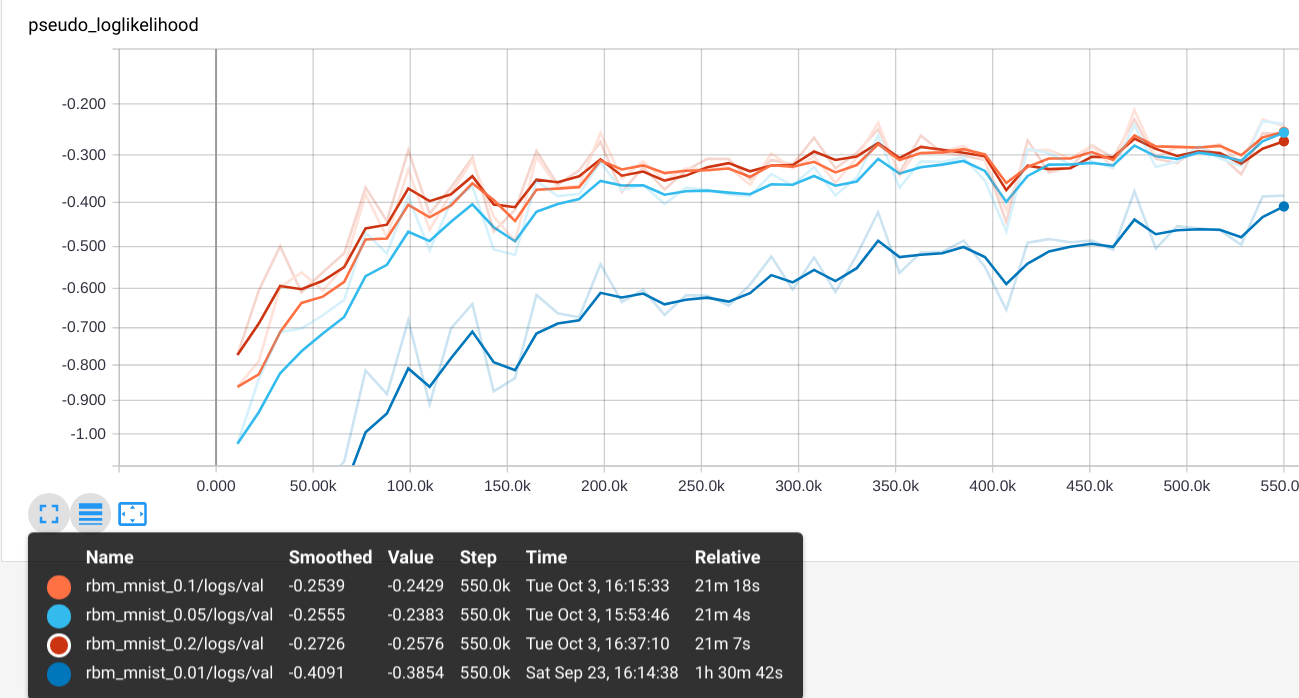
\includegraphics[width=5.6in]{rbm-mnist/pll_lr.png}
\\[2em]
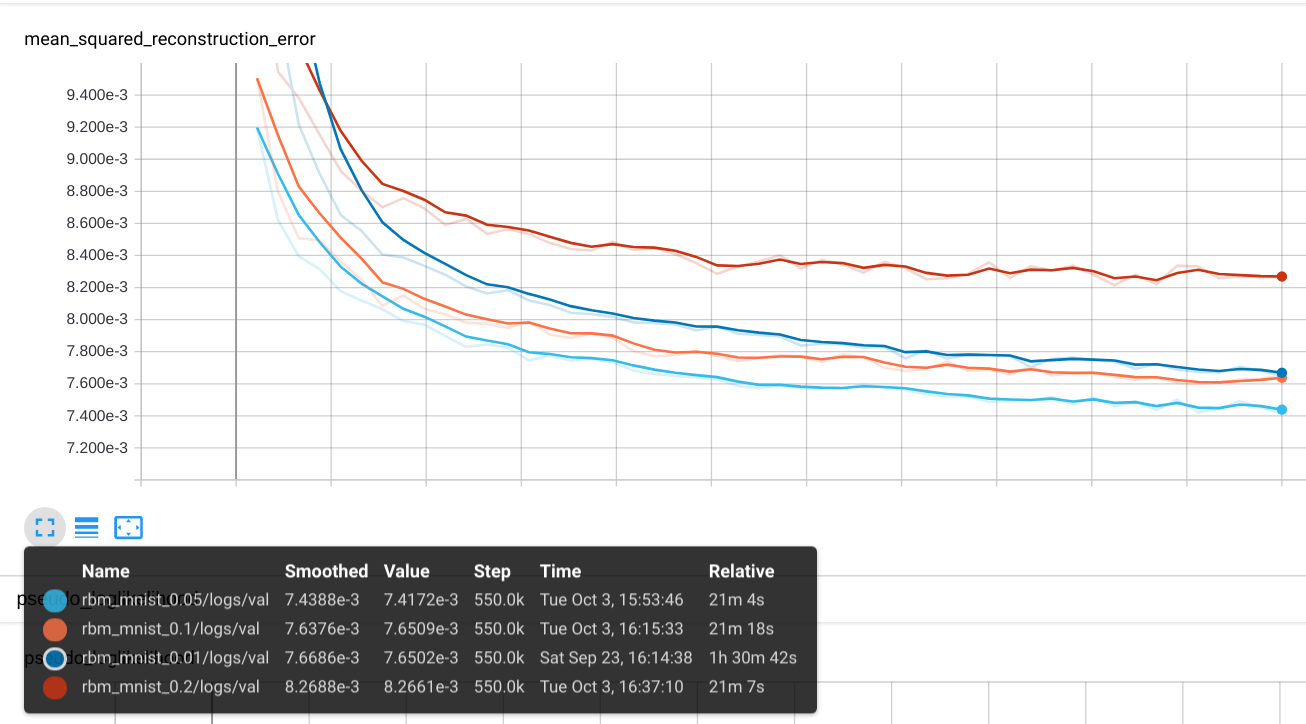
\includegraphics[width=5.6in]{rbm-mnist/msre_lr.png}
\caption{PLL and reconstruction error as learning rate varies (full MNIST).}
\end{mdframed}
\end{figure}

\clearpage

\begin{figure}[h]
\begin{mdframed}
\centering
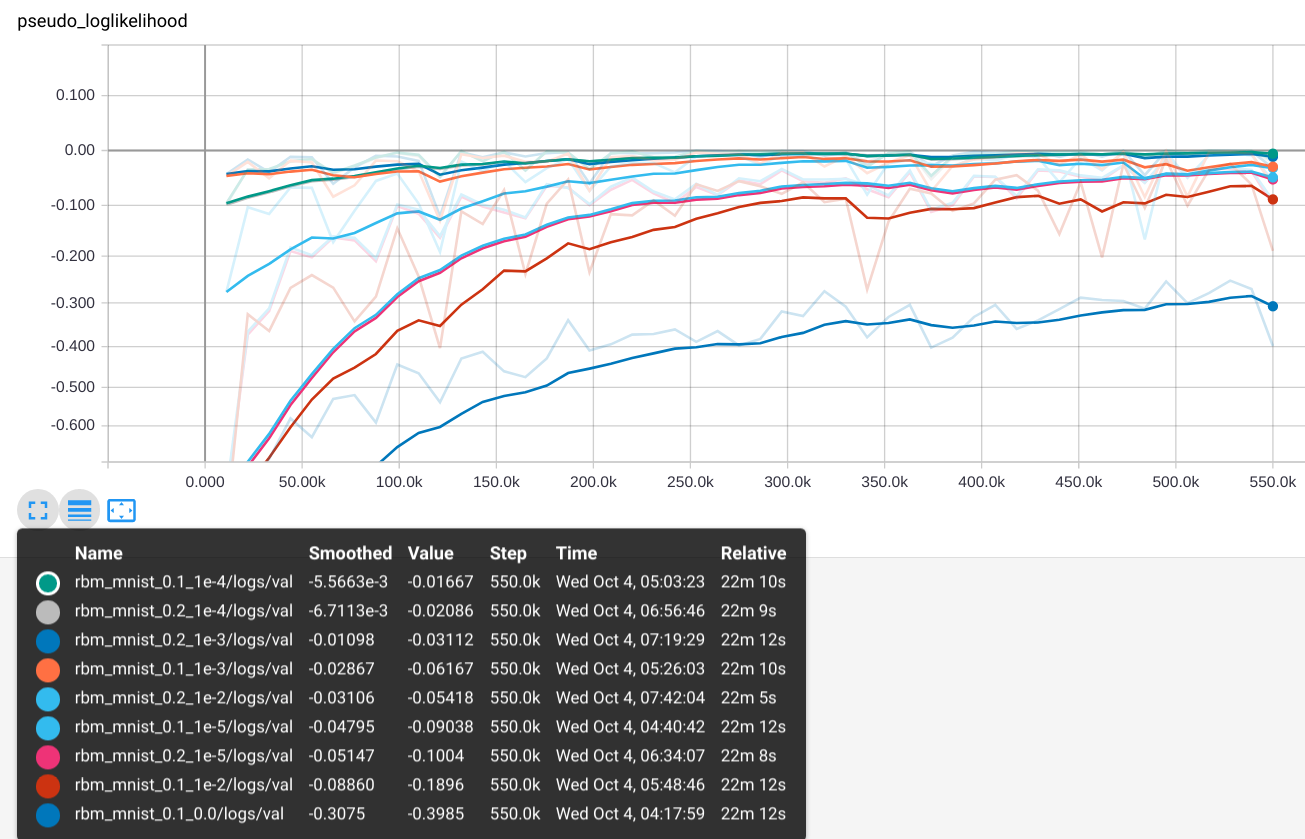
\includegraphics[width=5.6in]{rbm-mnist/st_pll.png}
\\[2em]
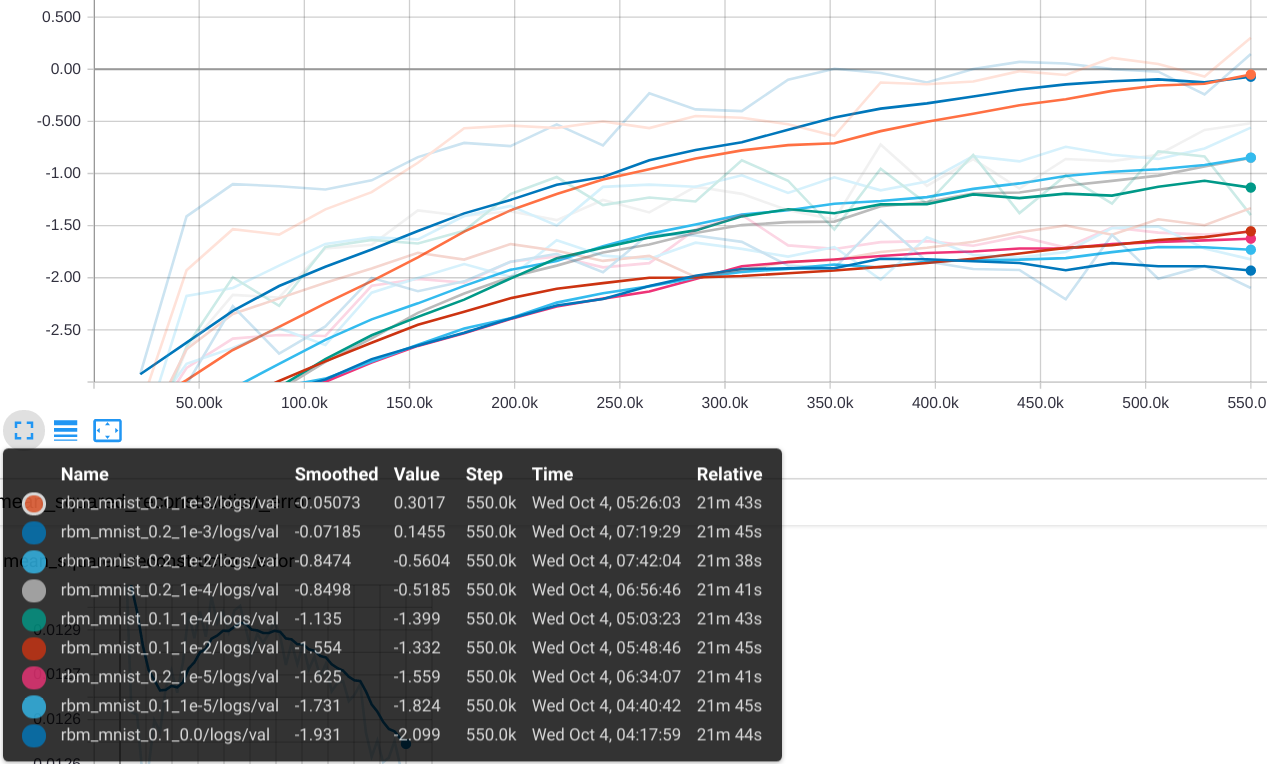
\includegraphics[width=5.6in]{rbm-mnist/st_feg.png}
\caption{PLL and free energy gap for sparsity target $t\in\{0,1\}$ and sparsity cost $\lambda \in \{0, 10^{-5\;\tb{:}\;-2}\}$ are used (full MNIST).}
\end{mdframed}
\end{figure}

\clearpage

\begin{figure}[h]
\begin{mdframed}
\centering
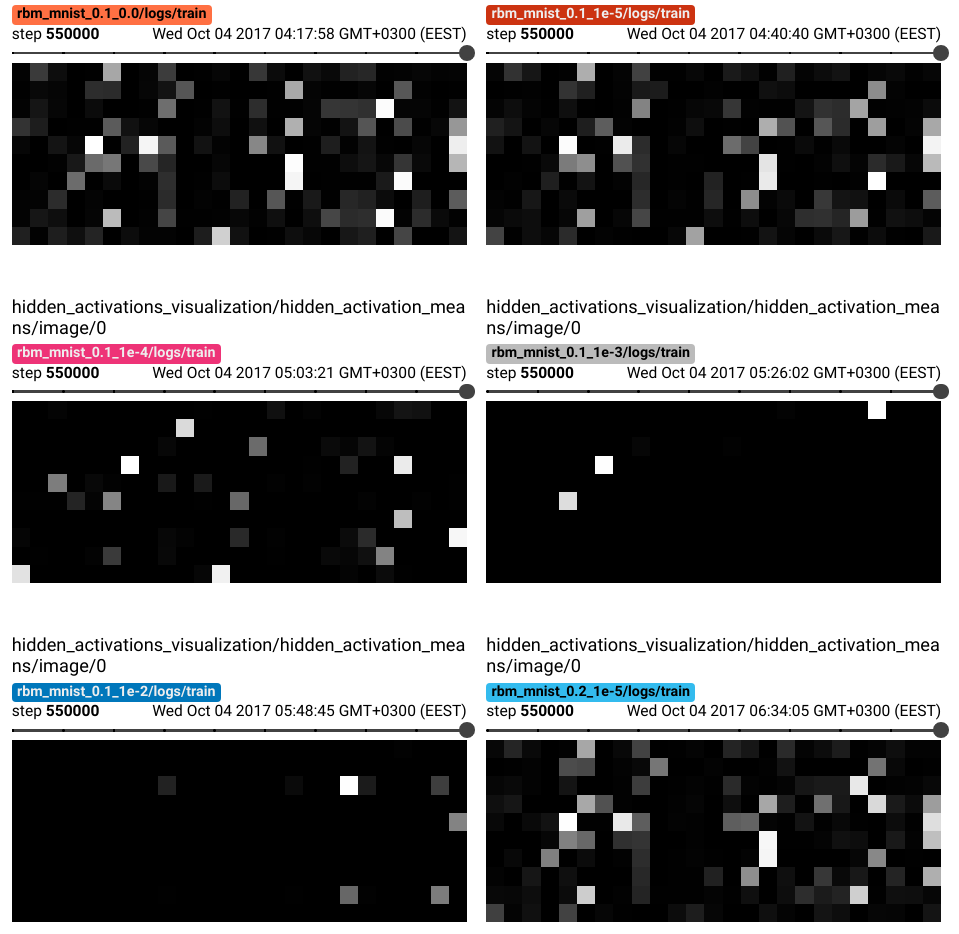
\includegraphics[width=4.8in]{rbm-mnist/st_hidden_activations.png}
\\[4em]
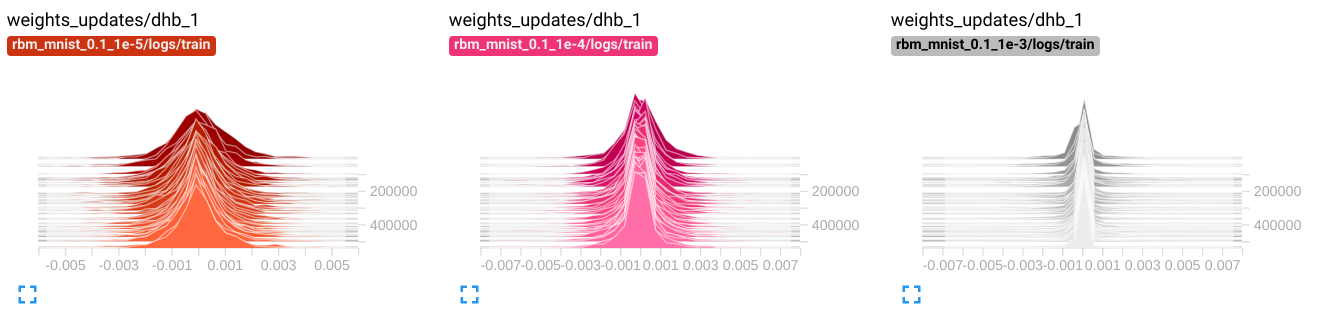
\includegraphics[width=5.6in]{rbm-mnist/st_hb_updates.png}
\caption{Hidden activations and hidden bias updates distributions from previous experiment. We clearly see that for larger $\lambda$ hidden activities become more and more sparse and distribtion becomes more and more peaky (same for weight updates).}
\end{mdframed}
\end{figure}

\clearpage

\begin{figure*}[t!]
\begin{mdframed}
\centering
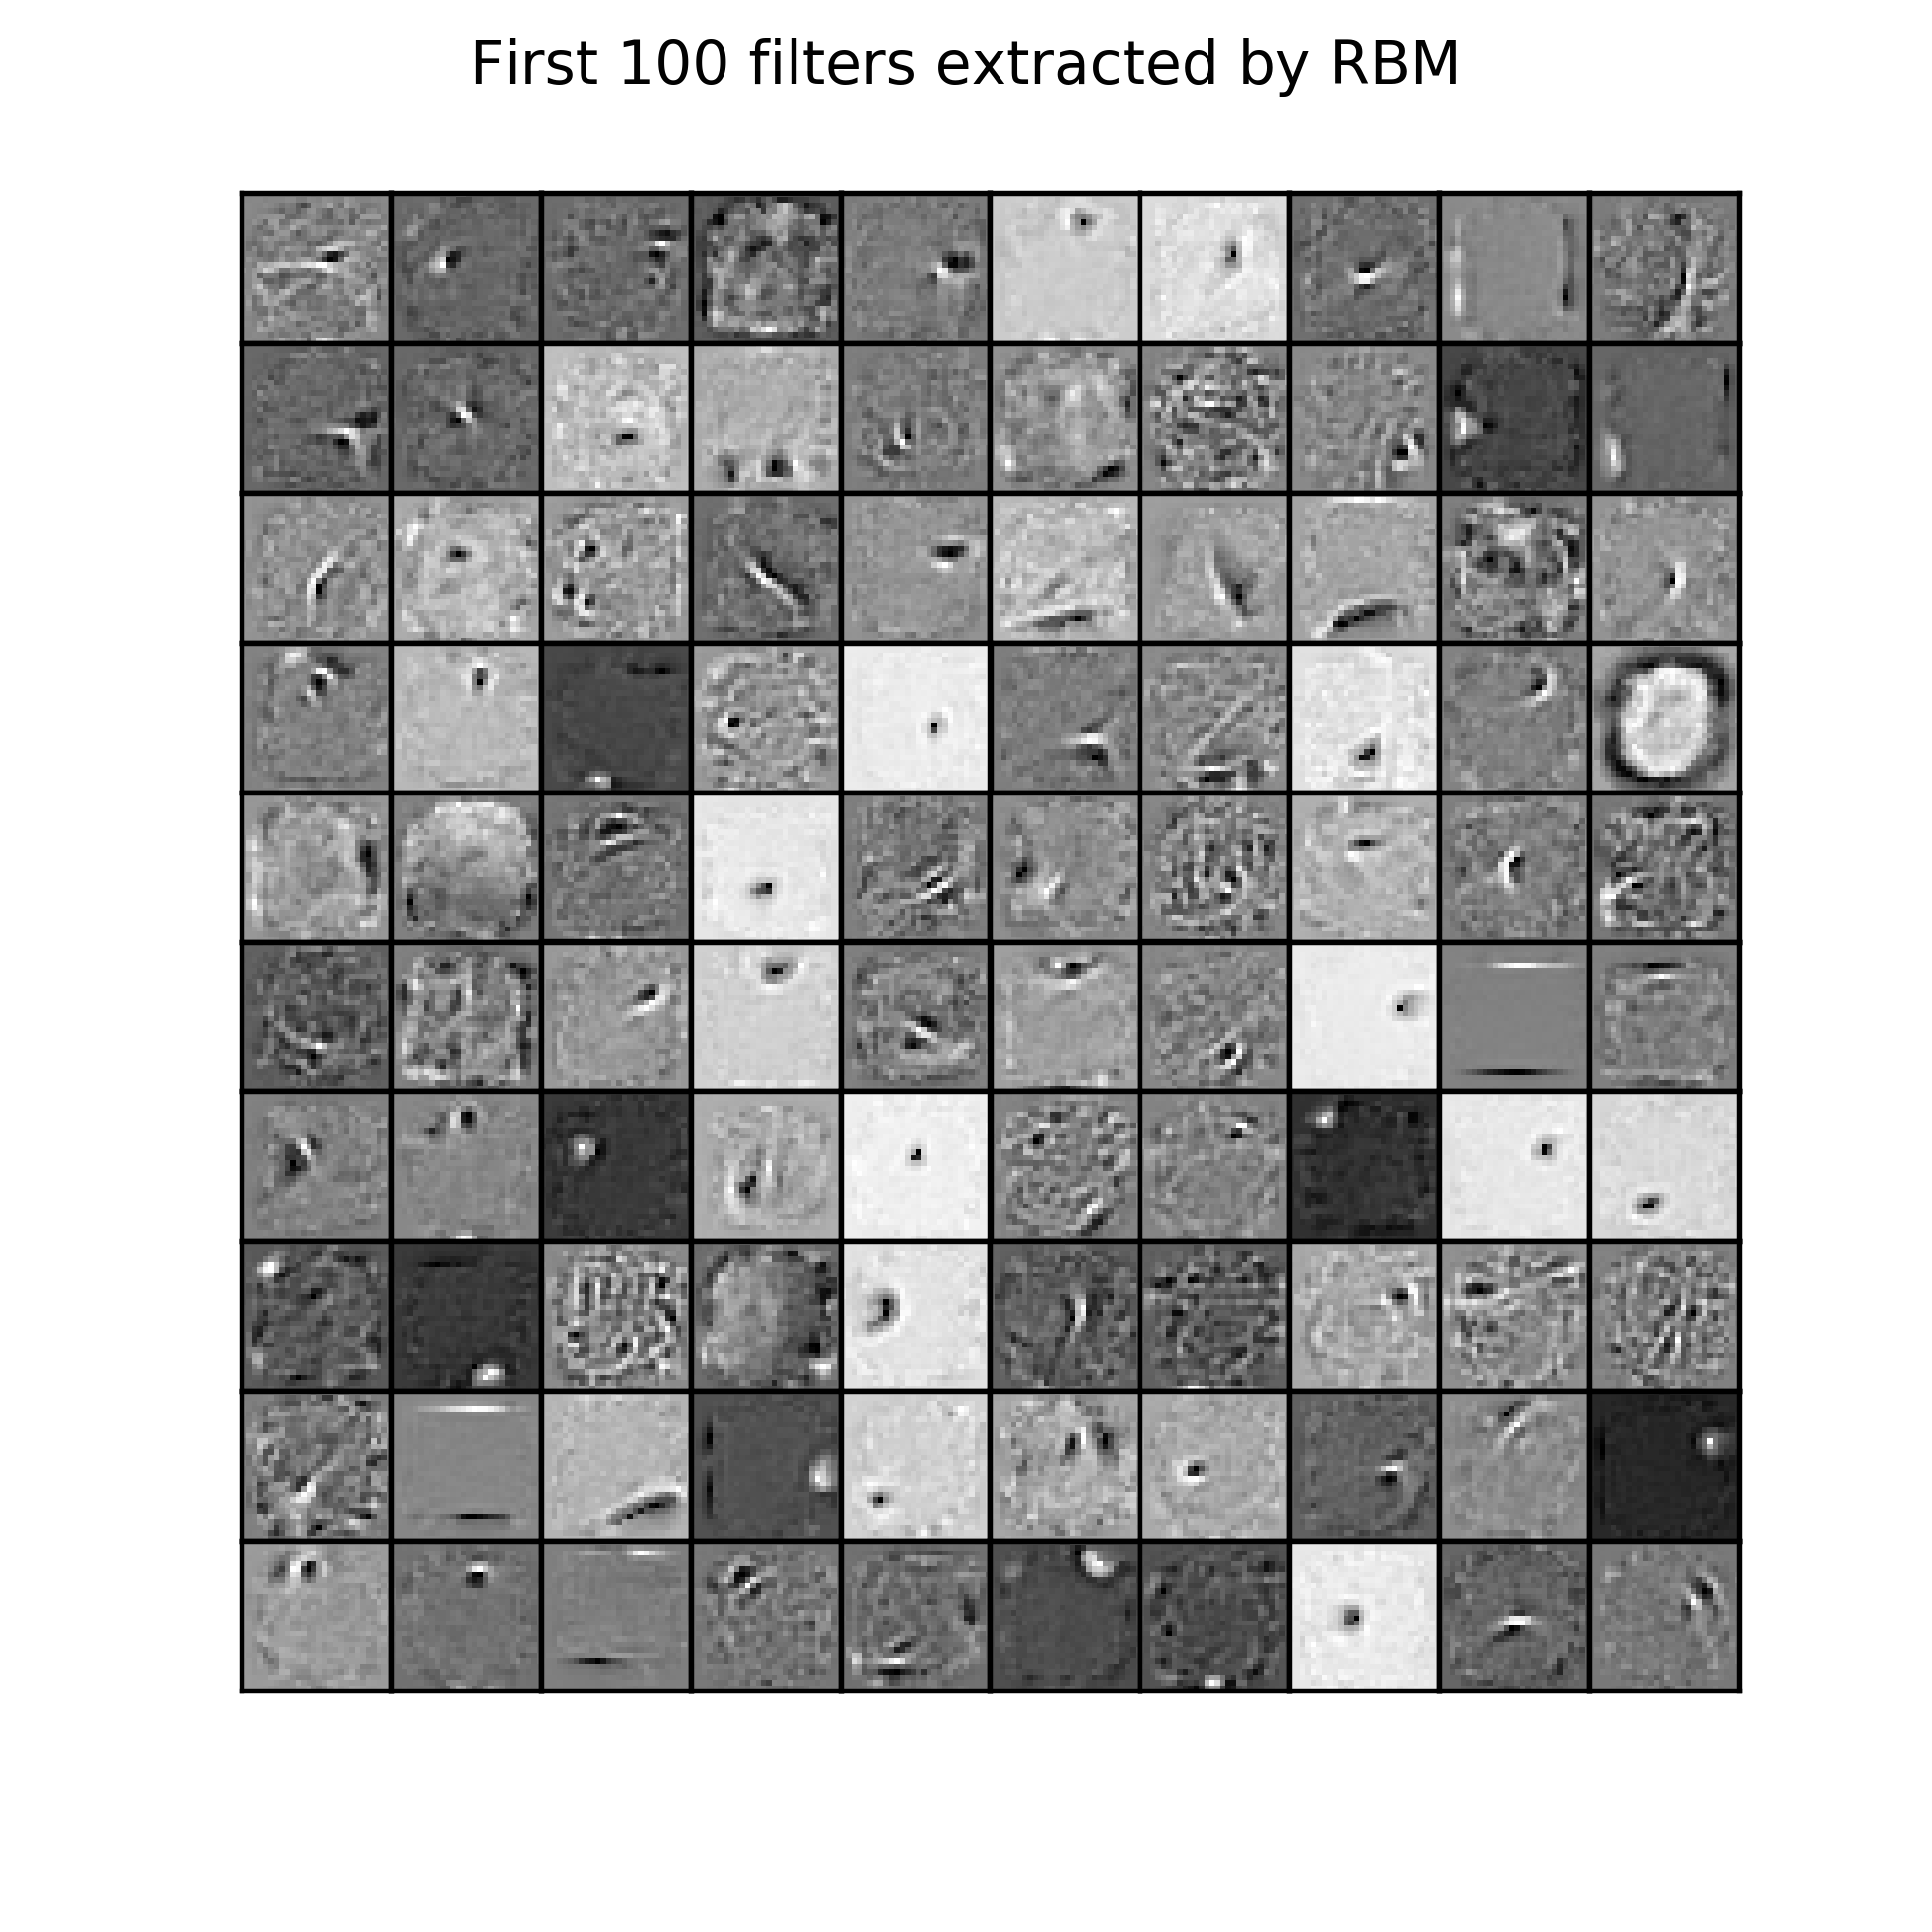
\includegraphics[width=.31\textwidth]{rbm-mnist/st_rbm_mnist_0.png}\quad
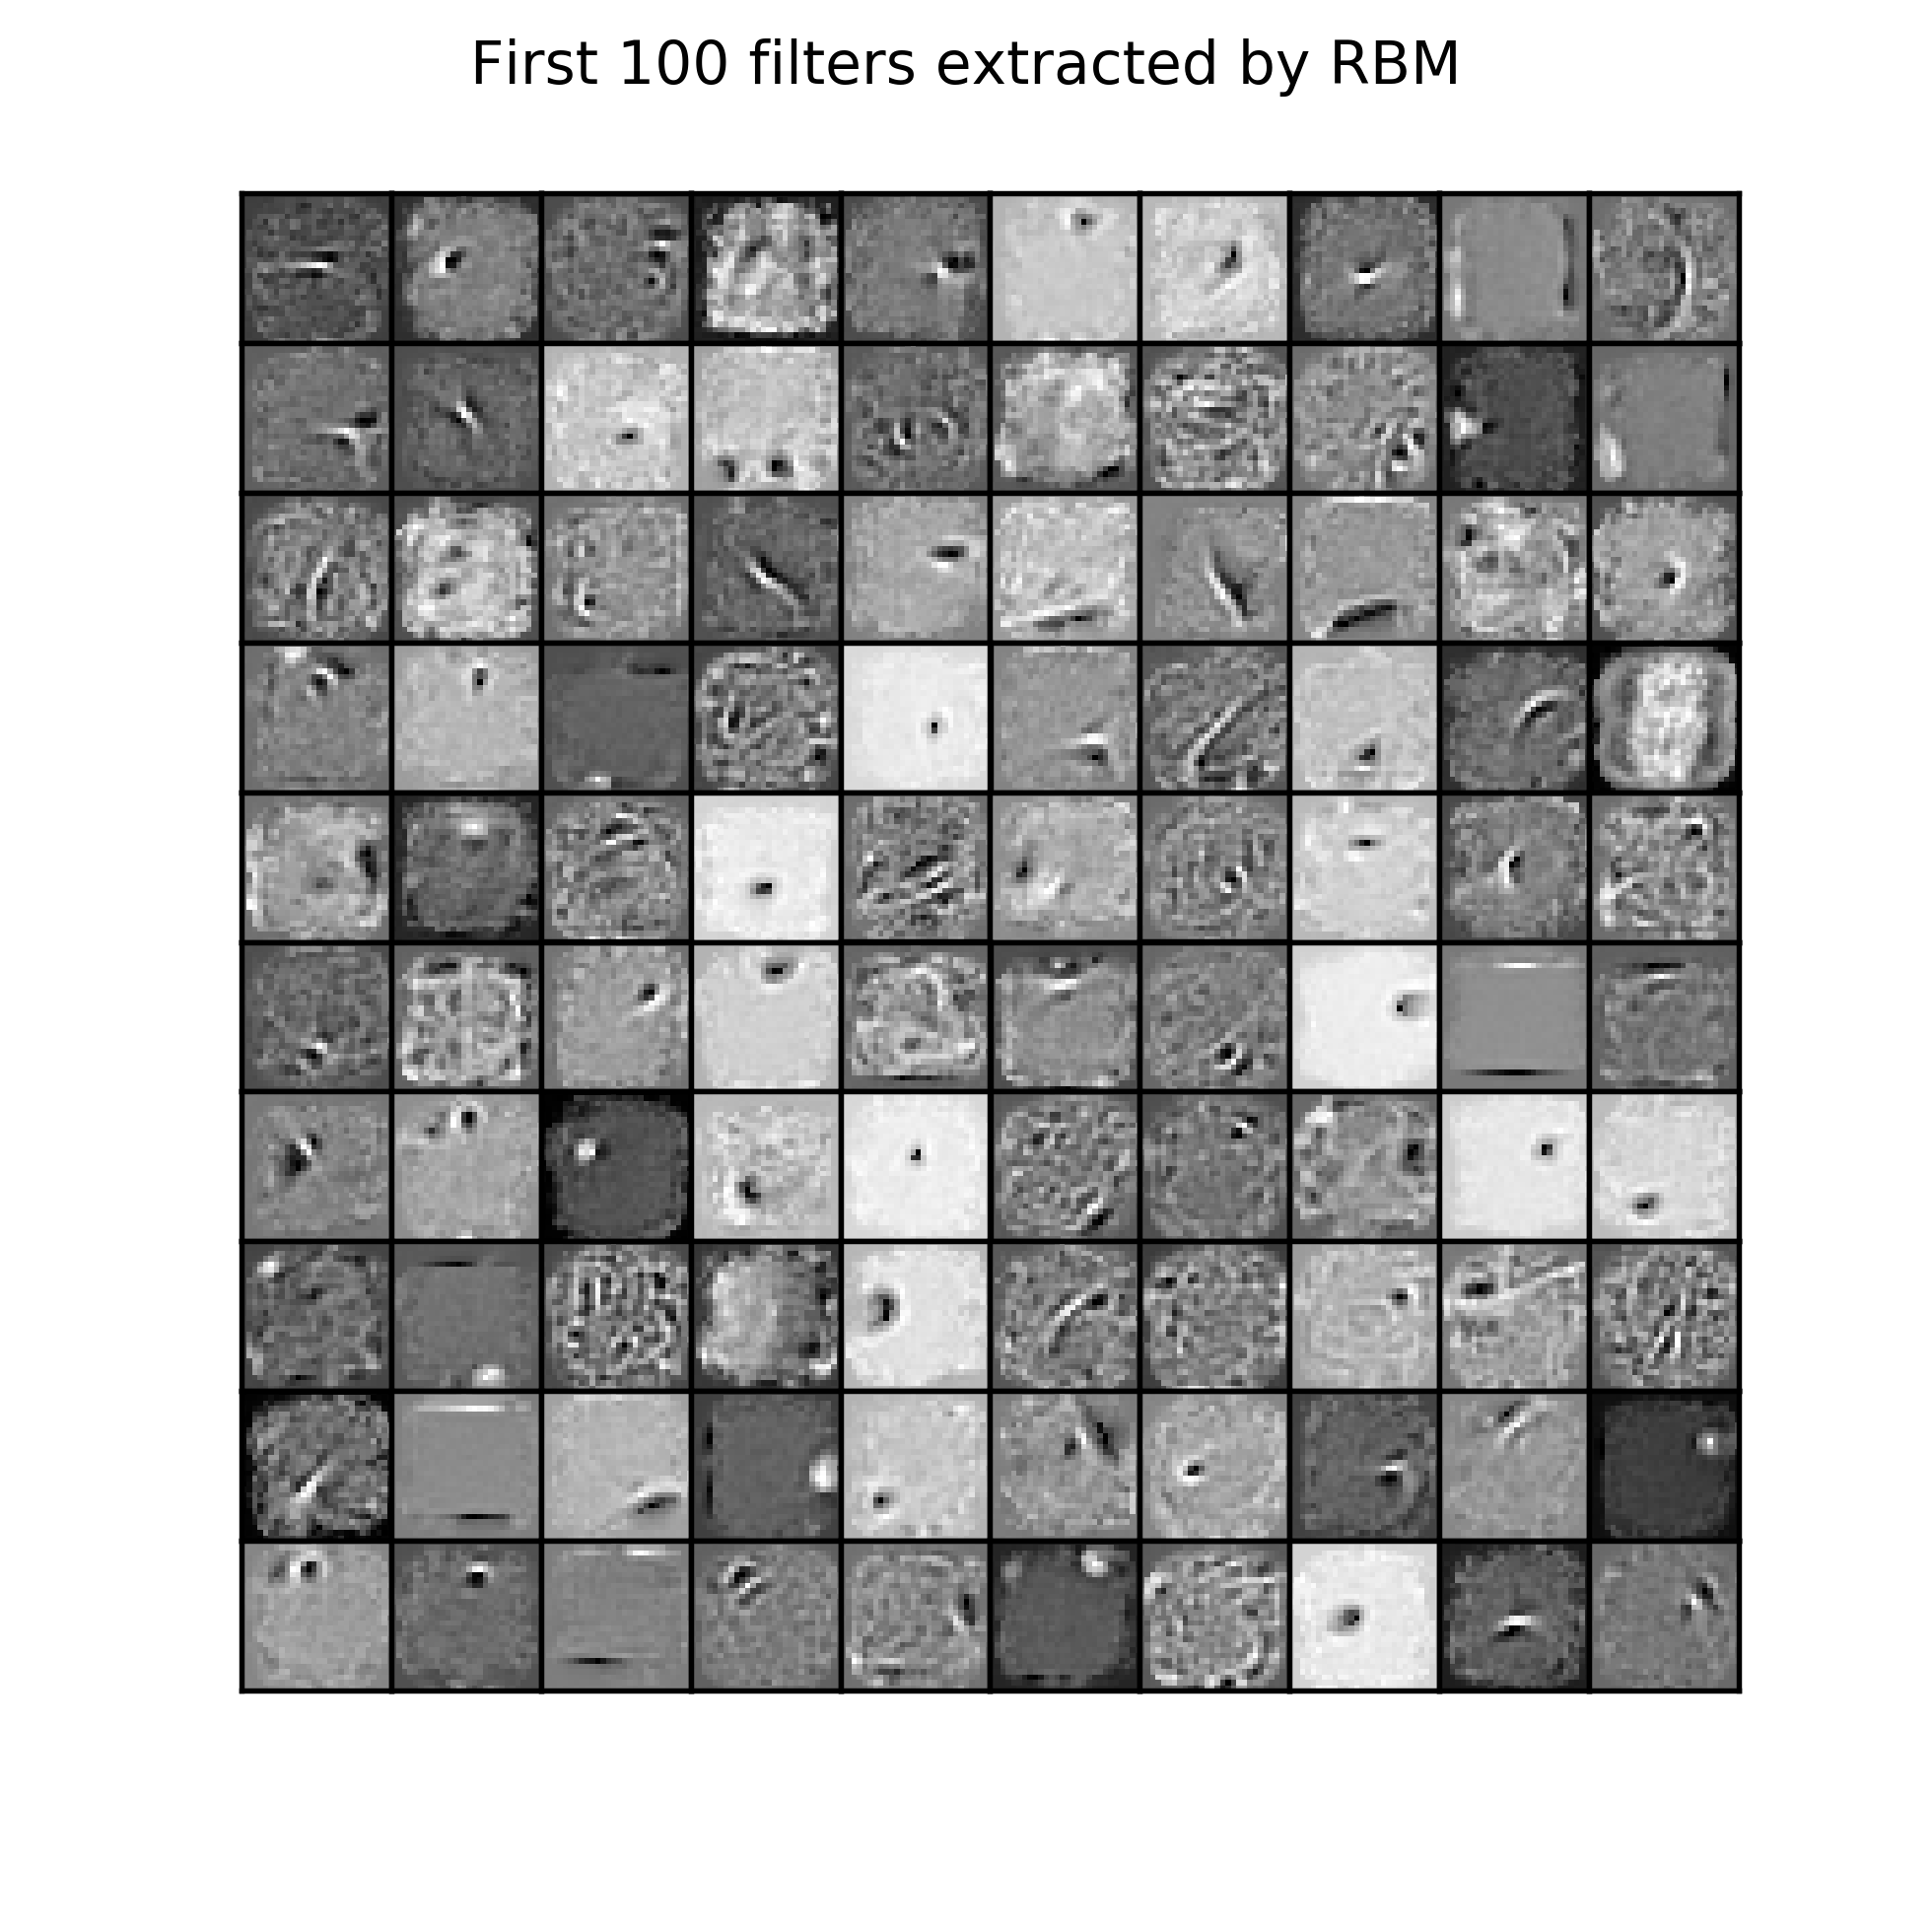
\includegraphics[width=.31\textwidth]{rbm-mnist/st_rbm_mnist_1e-5.png}\quad
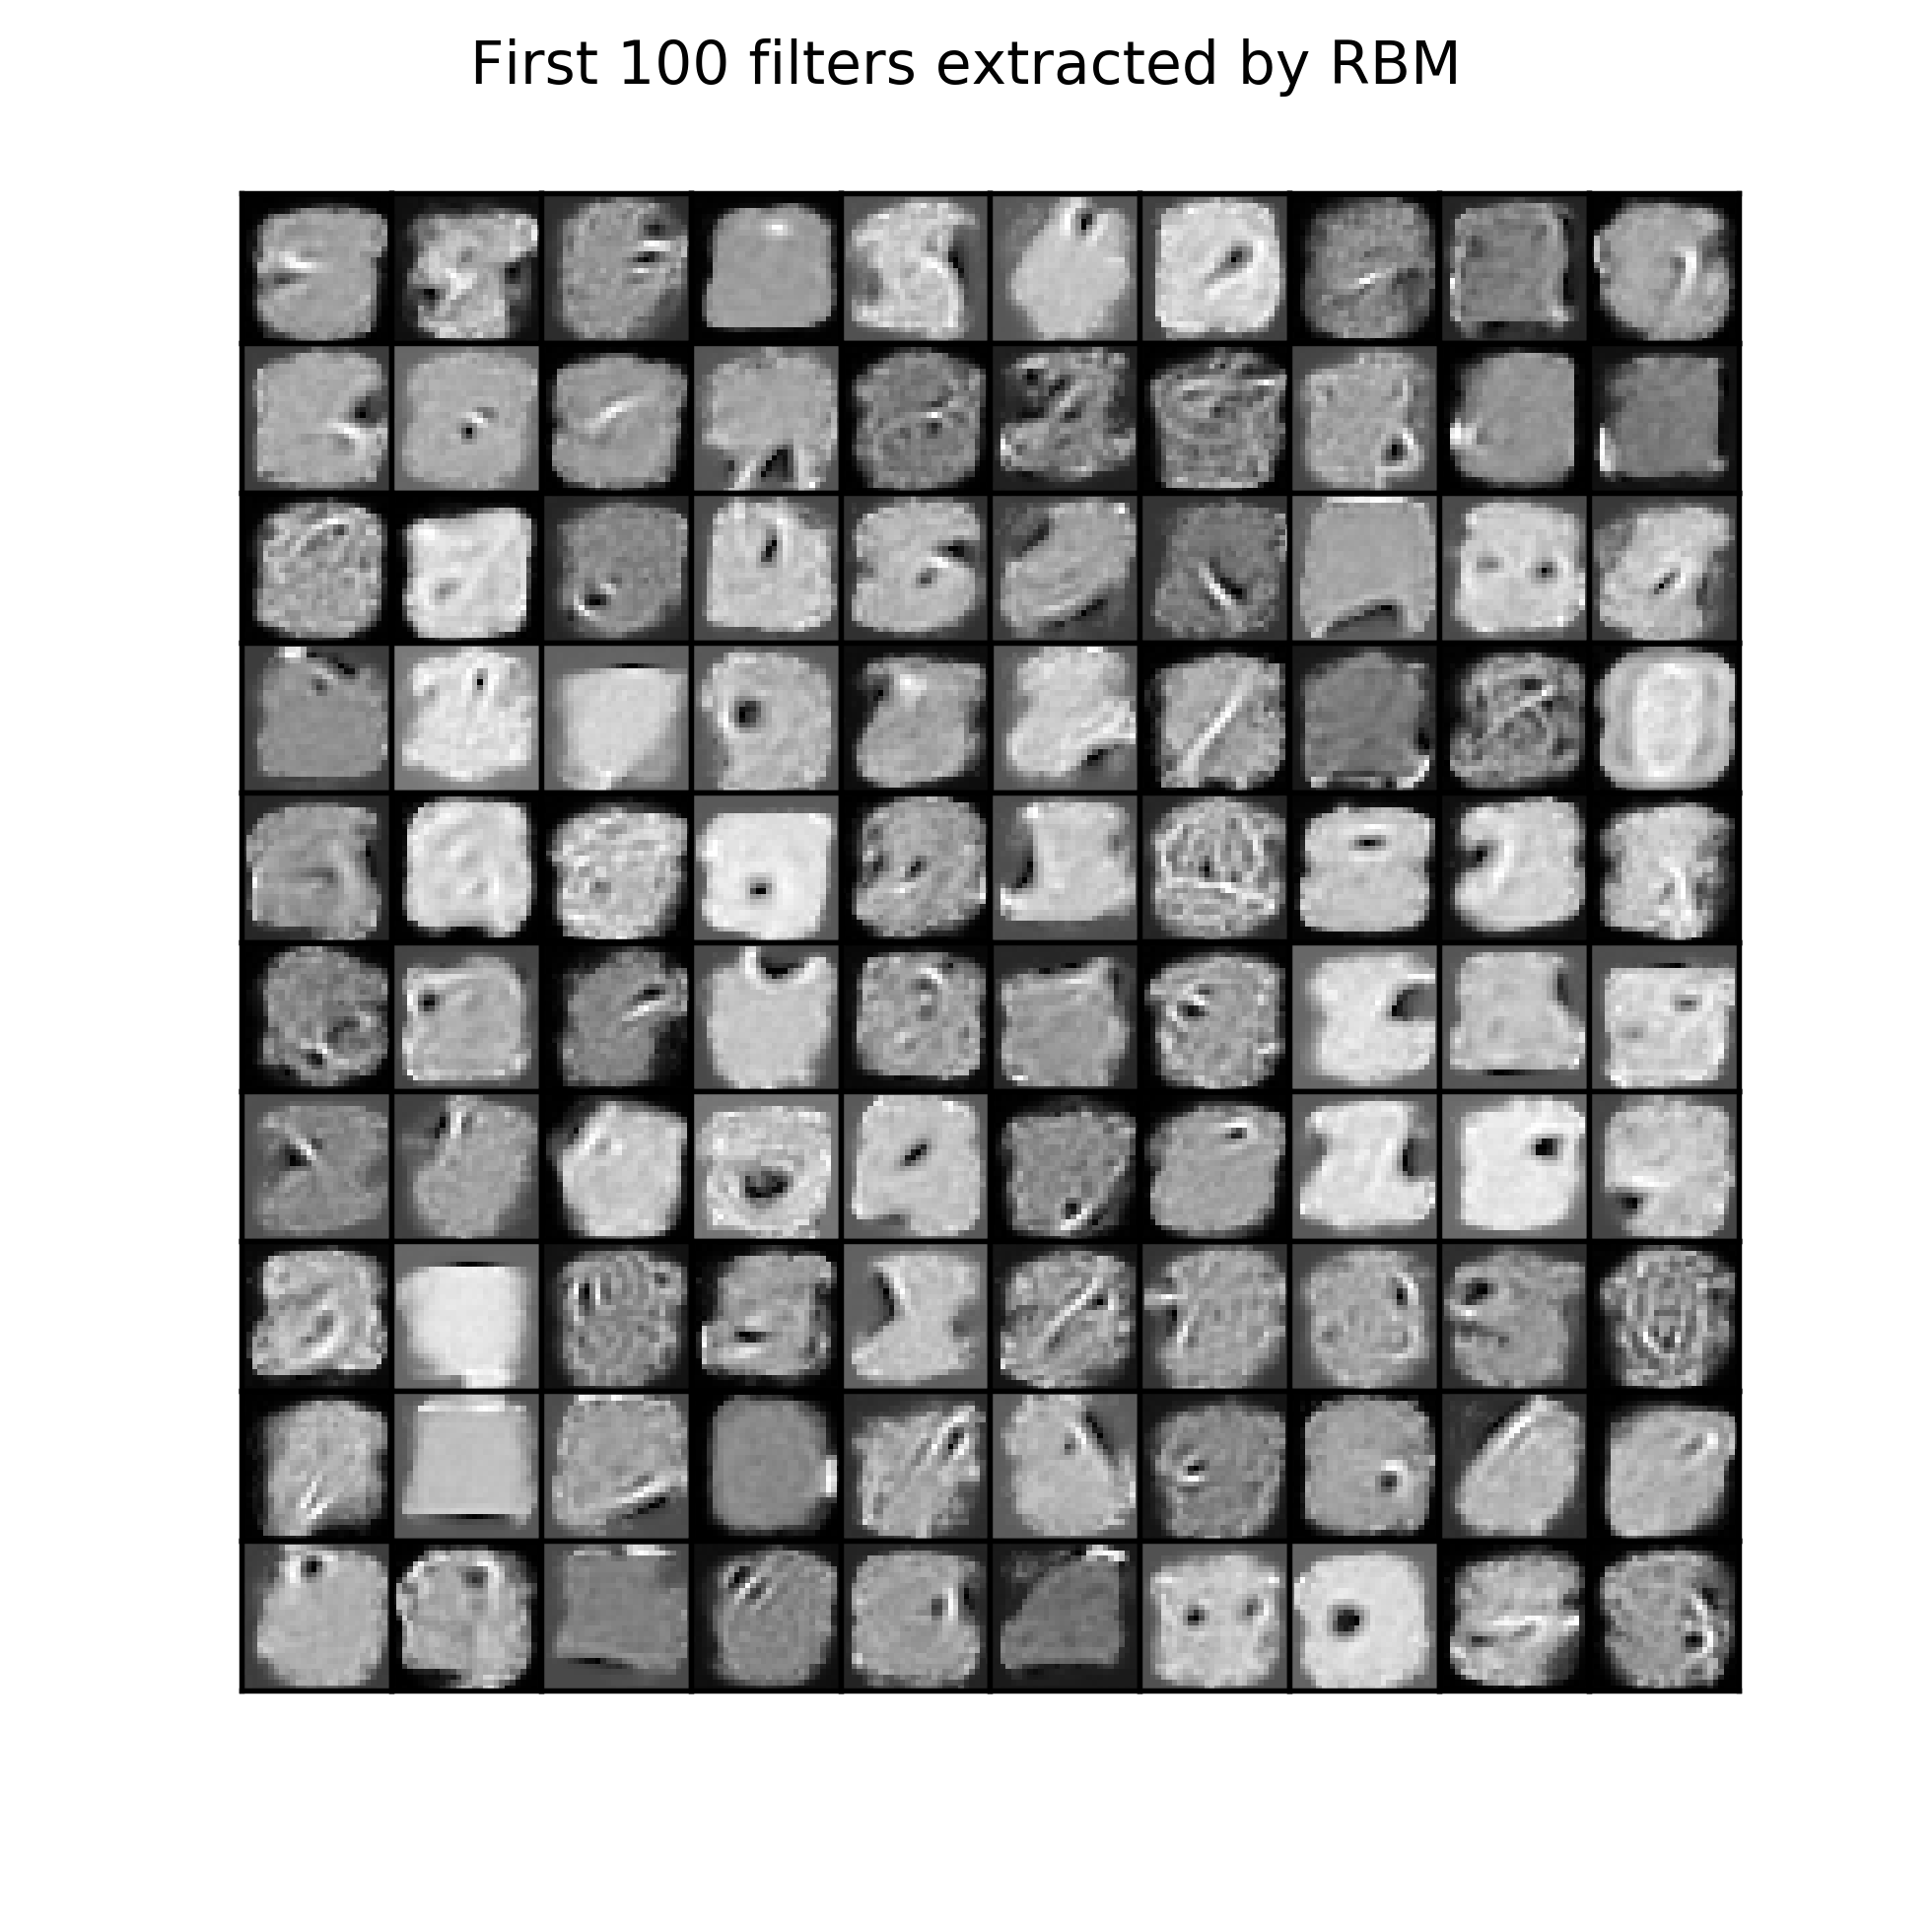
\includegraphics[width=.31\textwidth]{rbm-mnist/st_rbm_mnist_1e-4.png}

\medskip

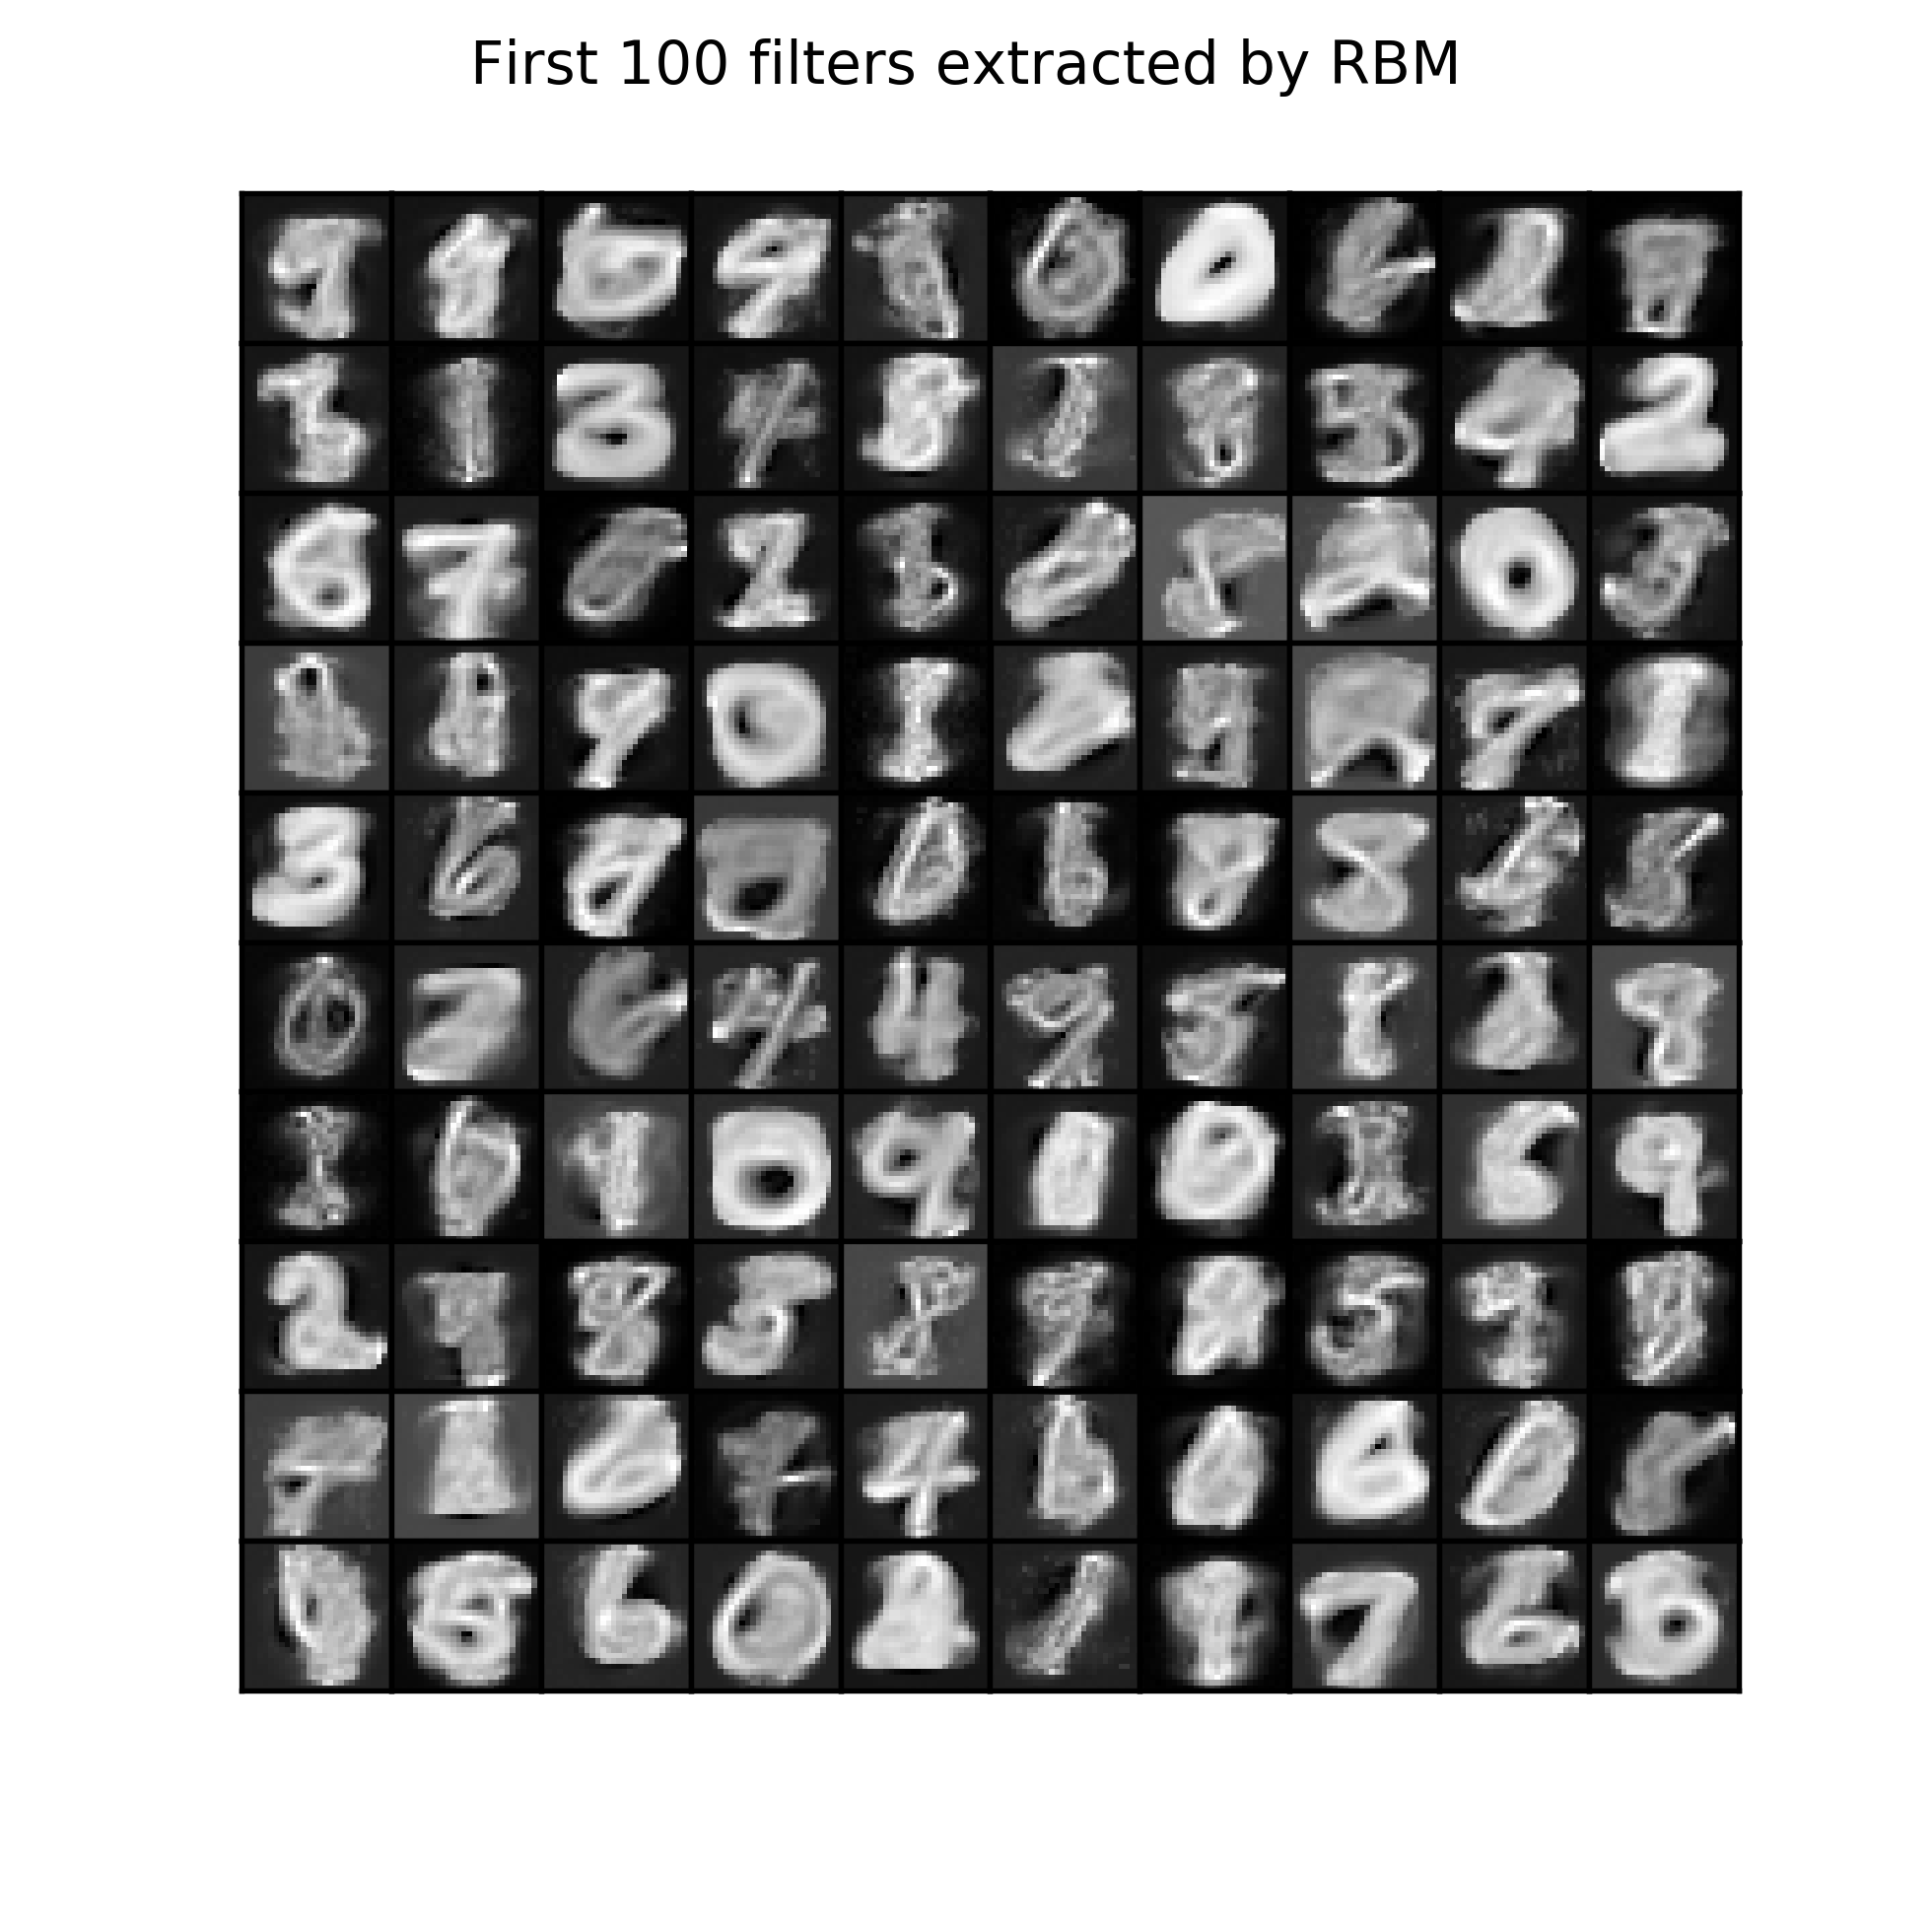
\includegraphics[width=.32\textwidth]{rbm-mnist/st_rbm_mnist_1e-3.png}\quad
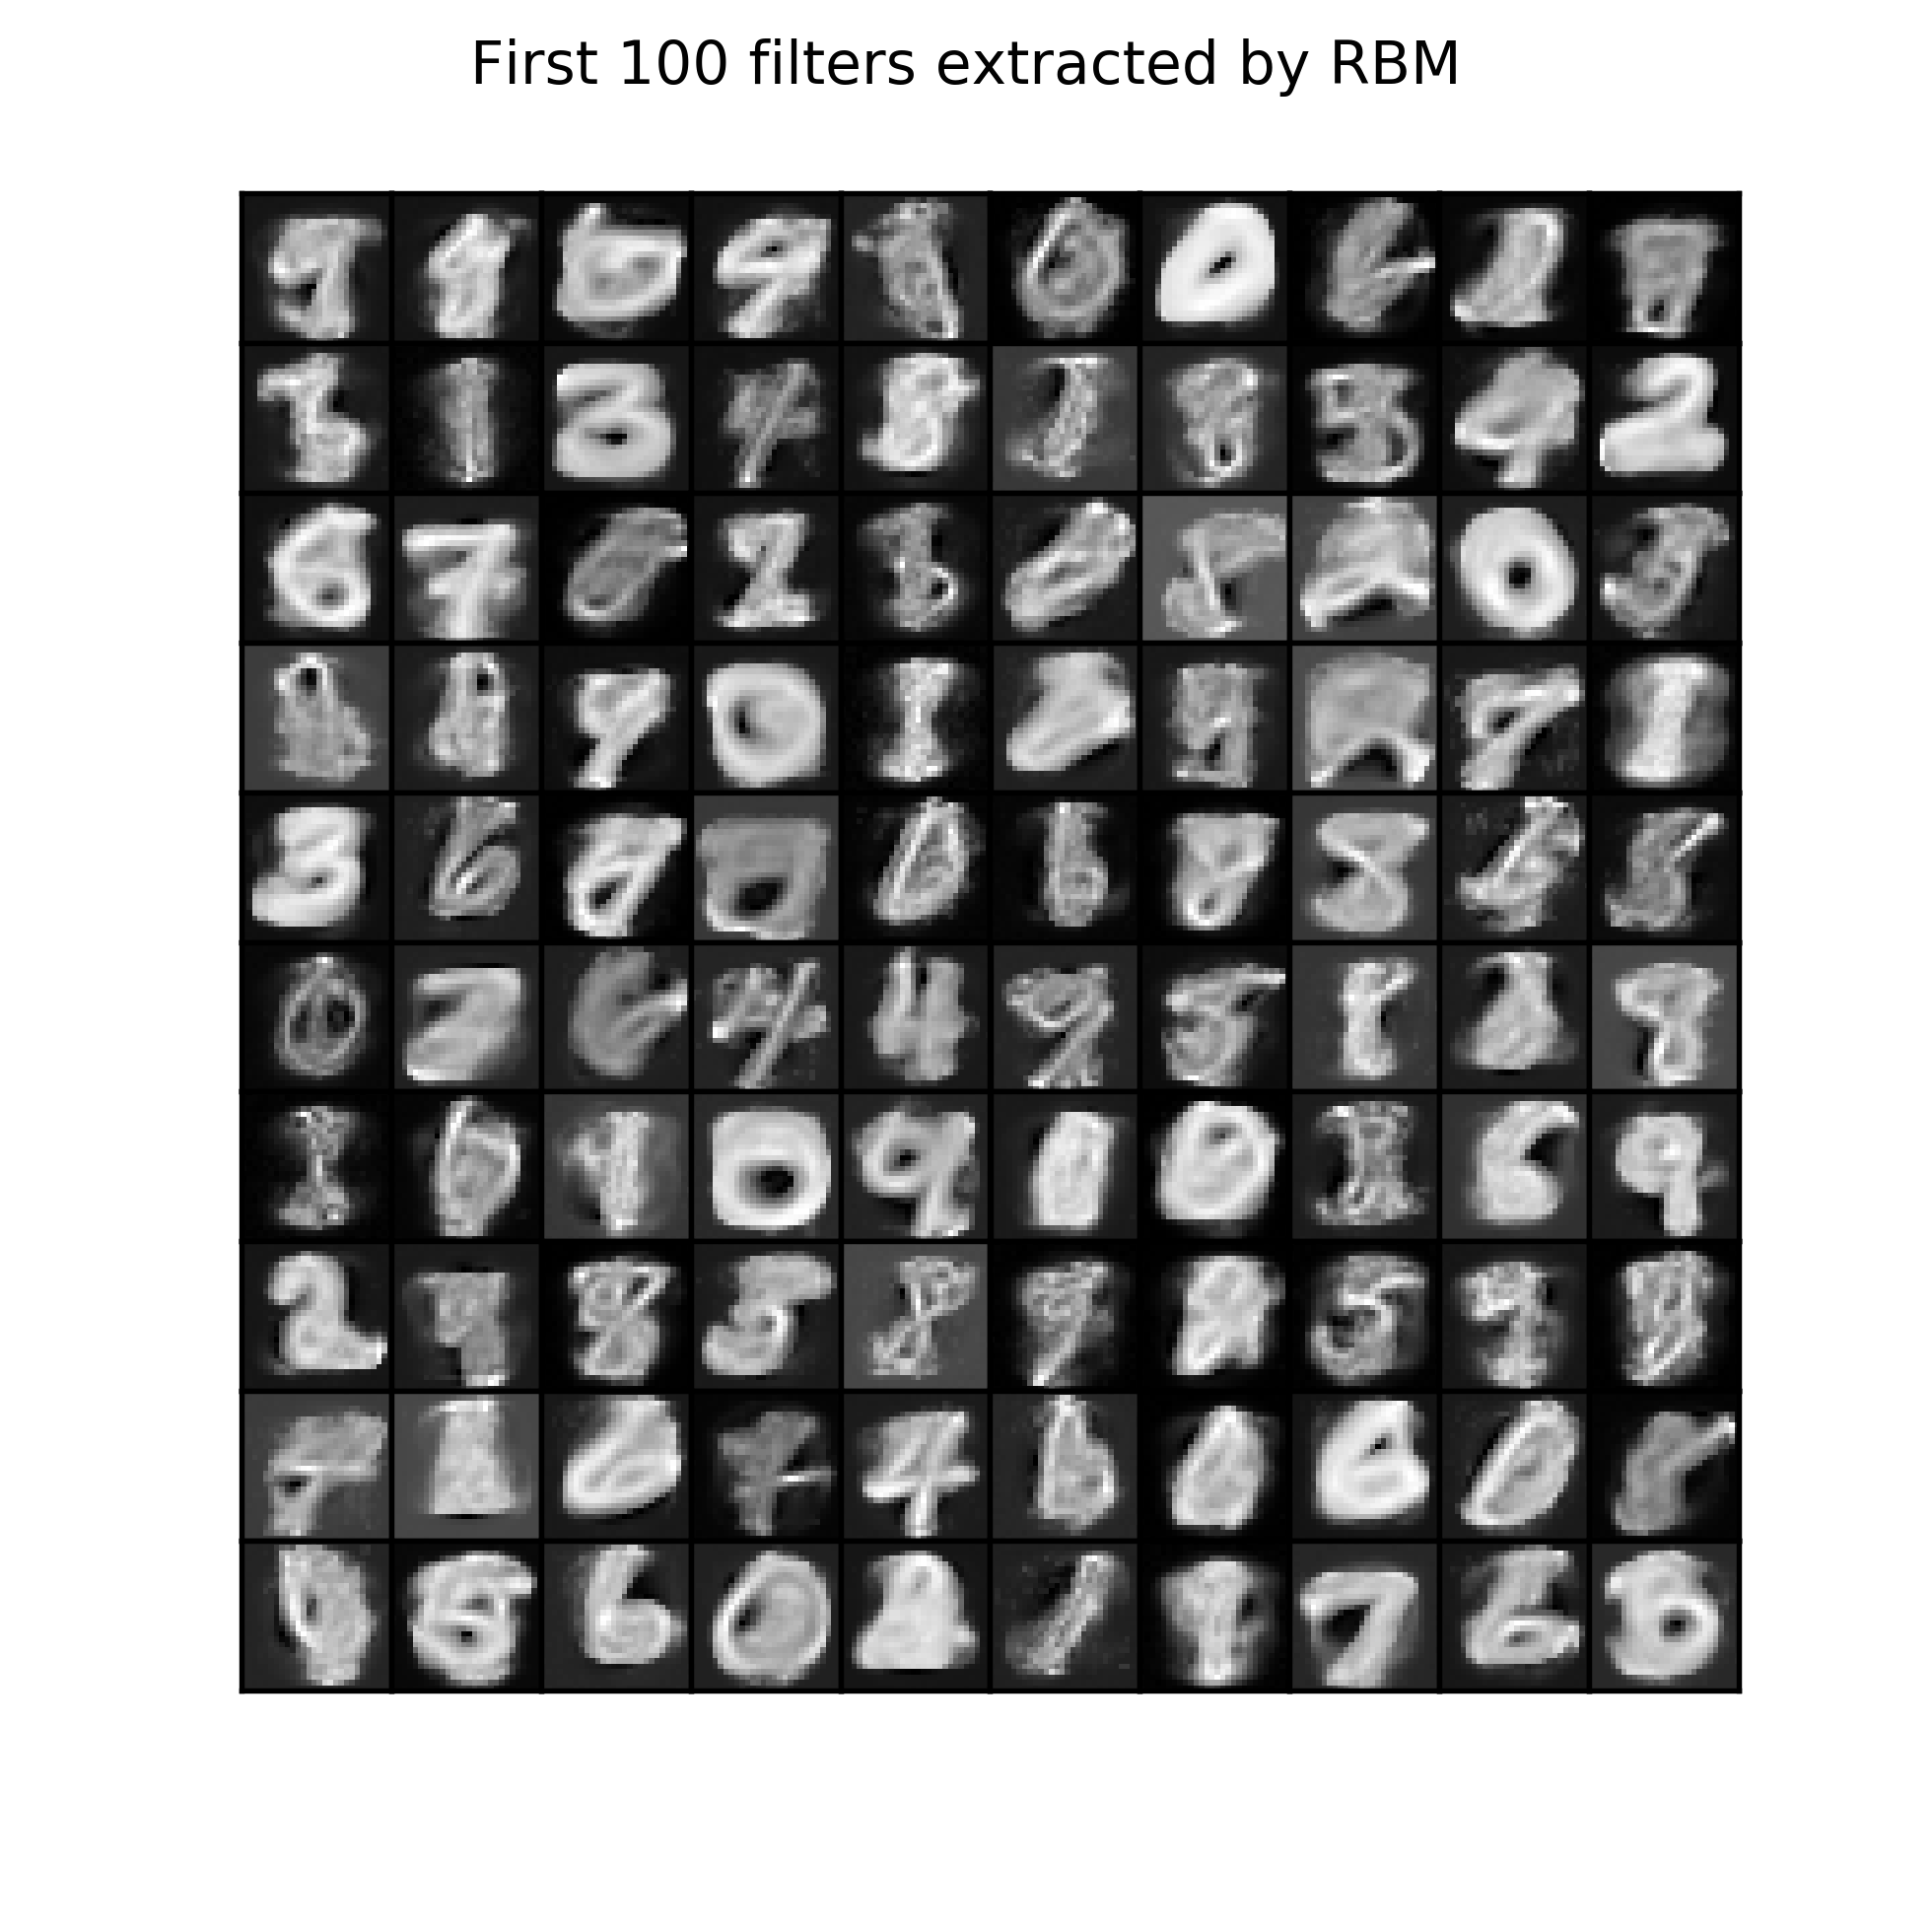
\includegraphics[width=.32\textwidth]{rbm-mnist/st_rbm_mnist_1e-3.png}

\medskip

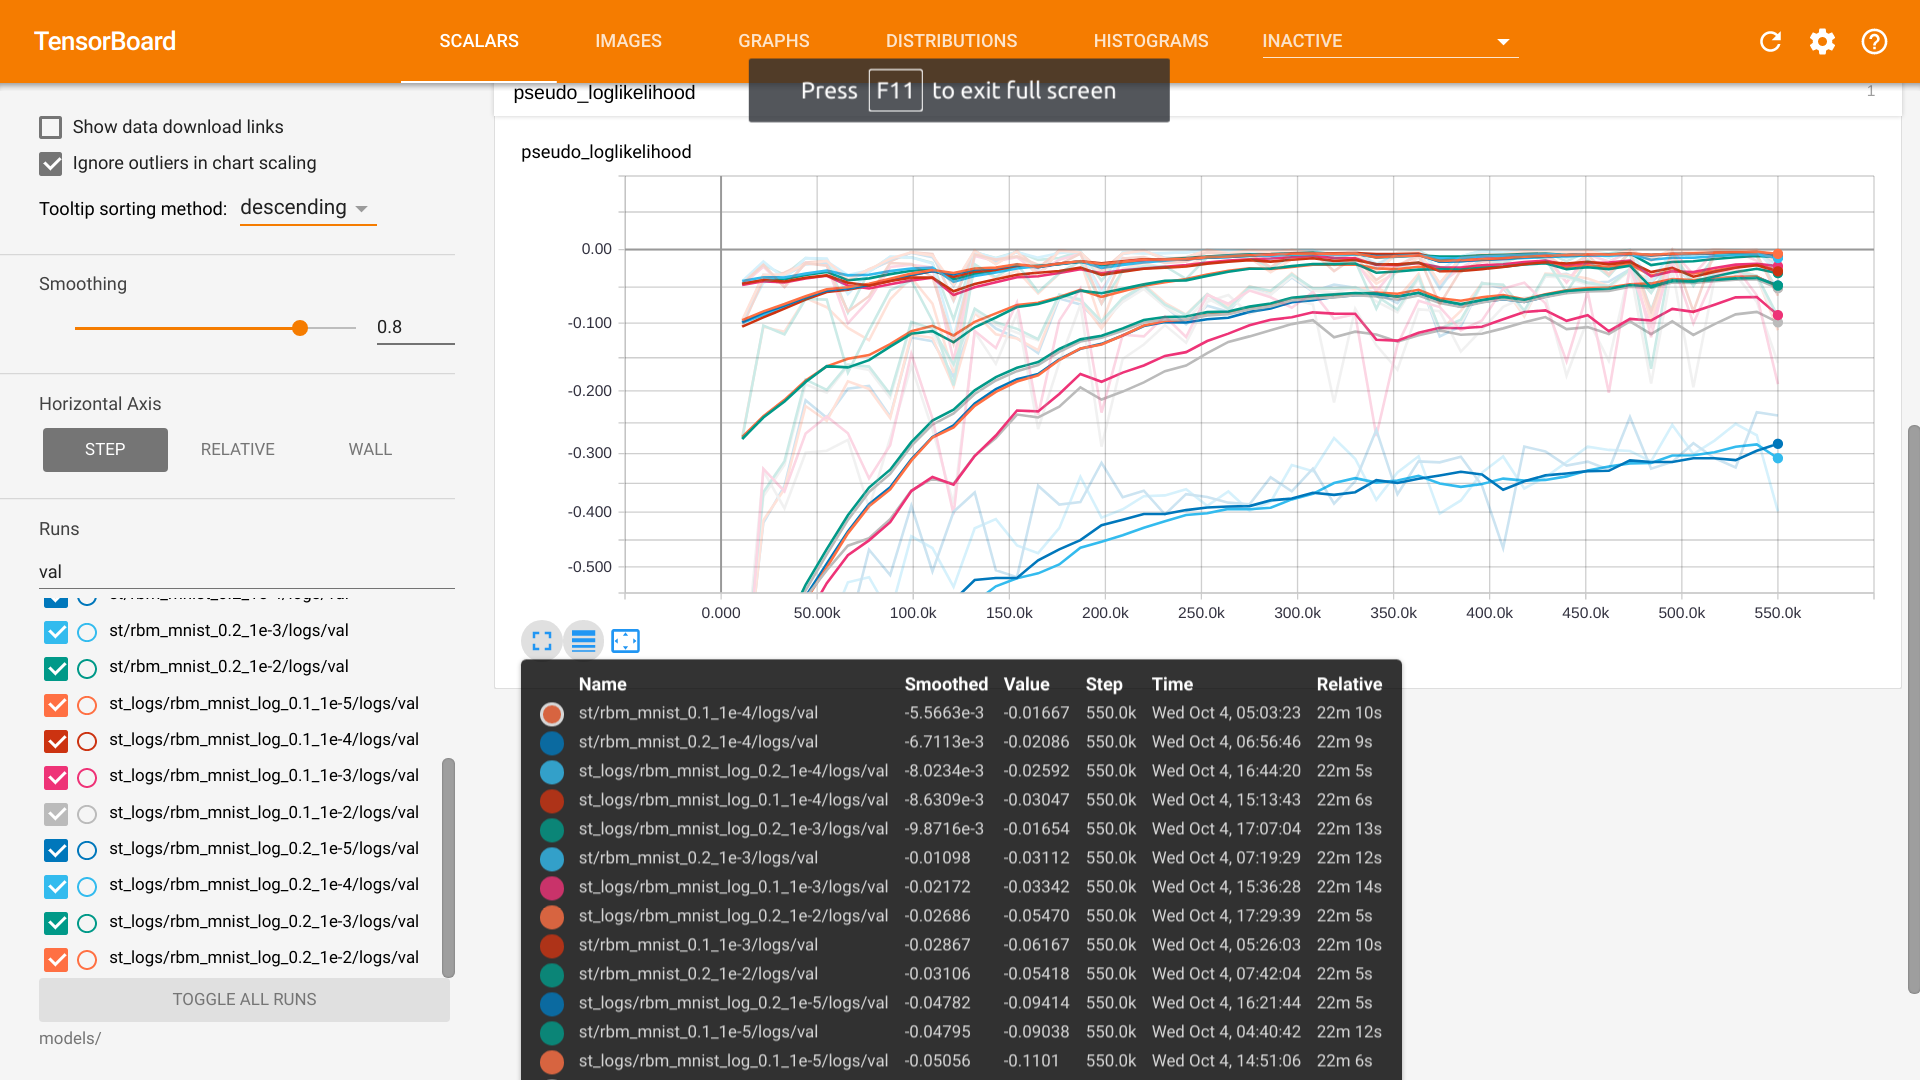
\includegraphics[width=.9\textwidth]{rbm-mnist/st_st_log_pll.png}
\caption{\emph{Top}: filters learned in the previous experiment as $\lambda$ increases (from top to bottom, from left to right). \emph{Bottom}: PLL of best models from previous experiment and ones with hidden biases initialized as $\log\l(\frac{t}{1-t}\r)$ for sparsity target $t$.}
\end{mdframed}
\end{figure*}

\clearpage

\begin{figure}[h]
\begin{mdframed}
\centering
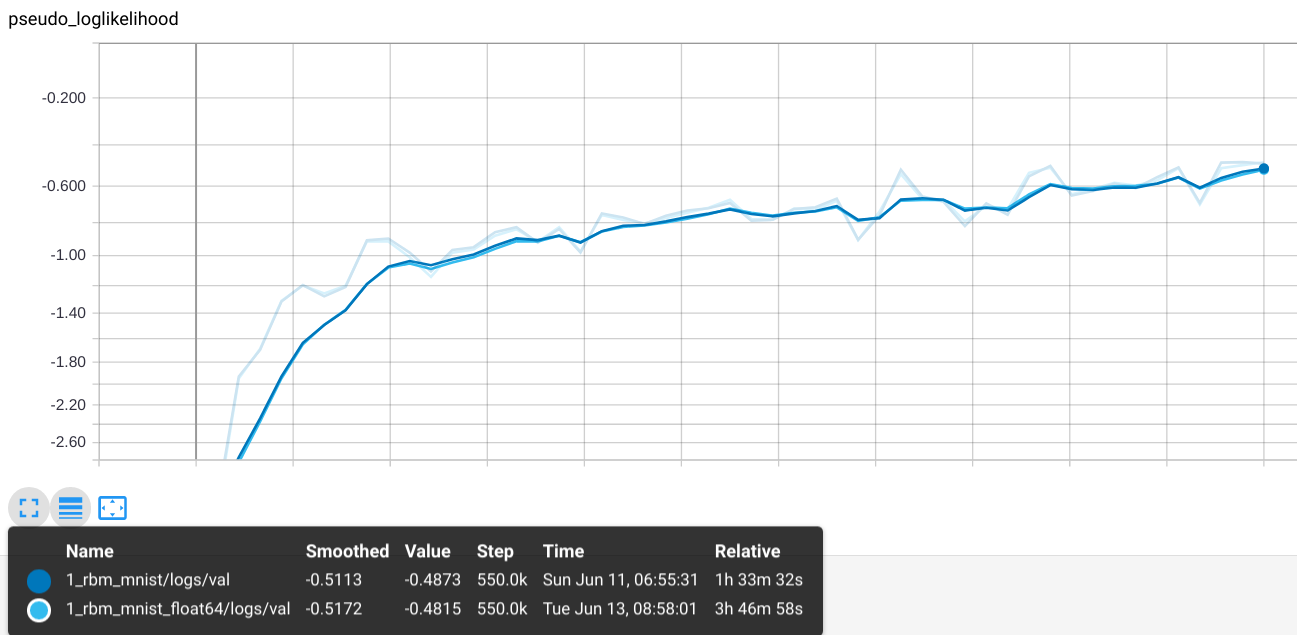
\includegraphics[width=5.8in]{rbm-mnist/float32_float64.png}
\\[1em]
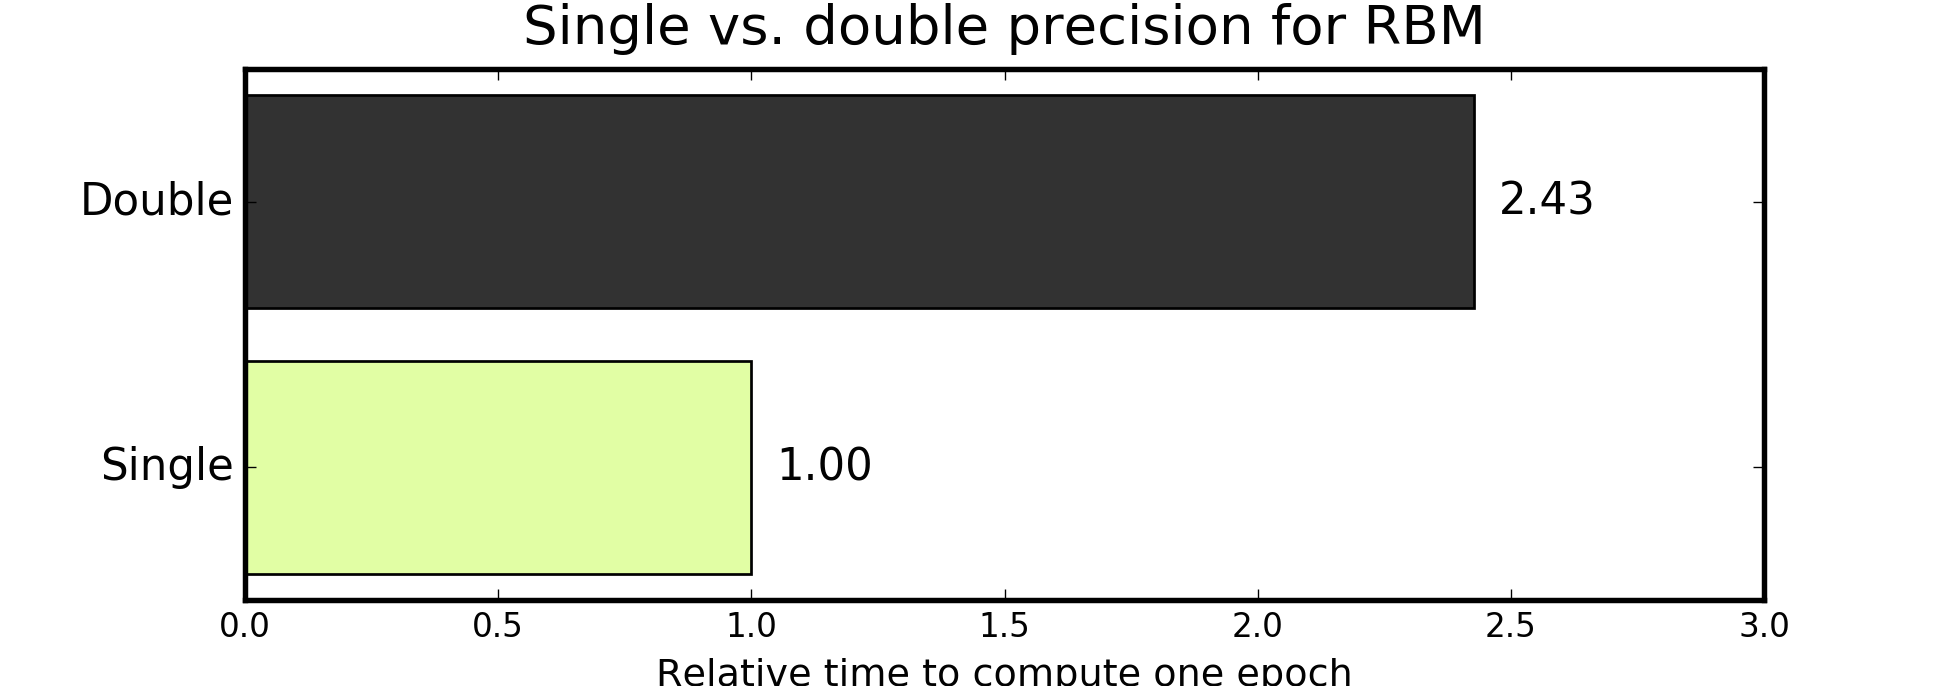
\includegraphics[width=3in]{rbm-mnist/rbm_speedup.png}
\\[1em]
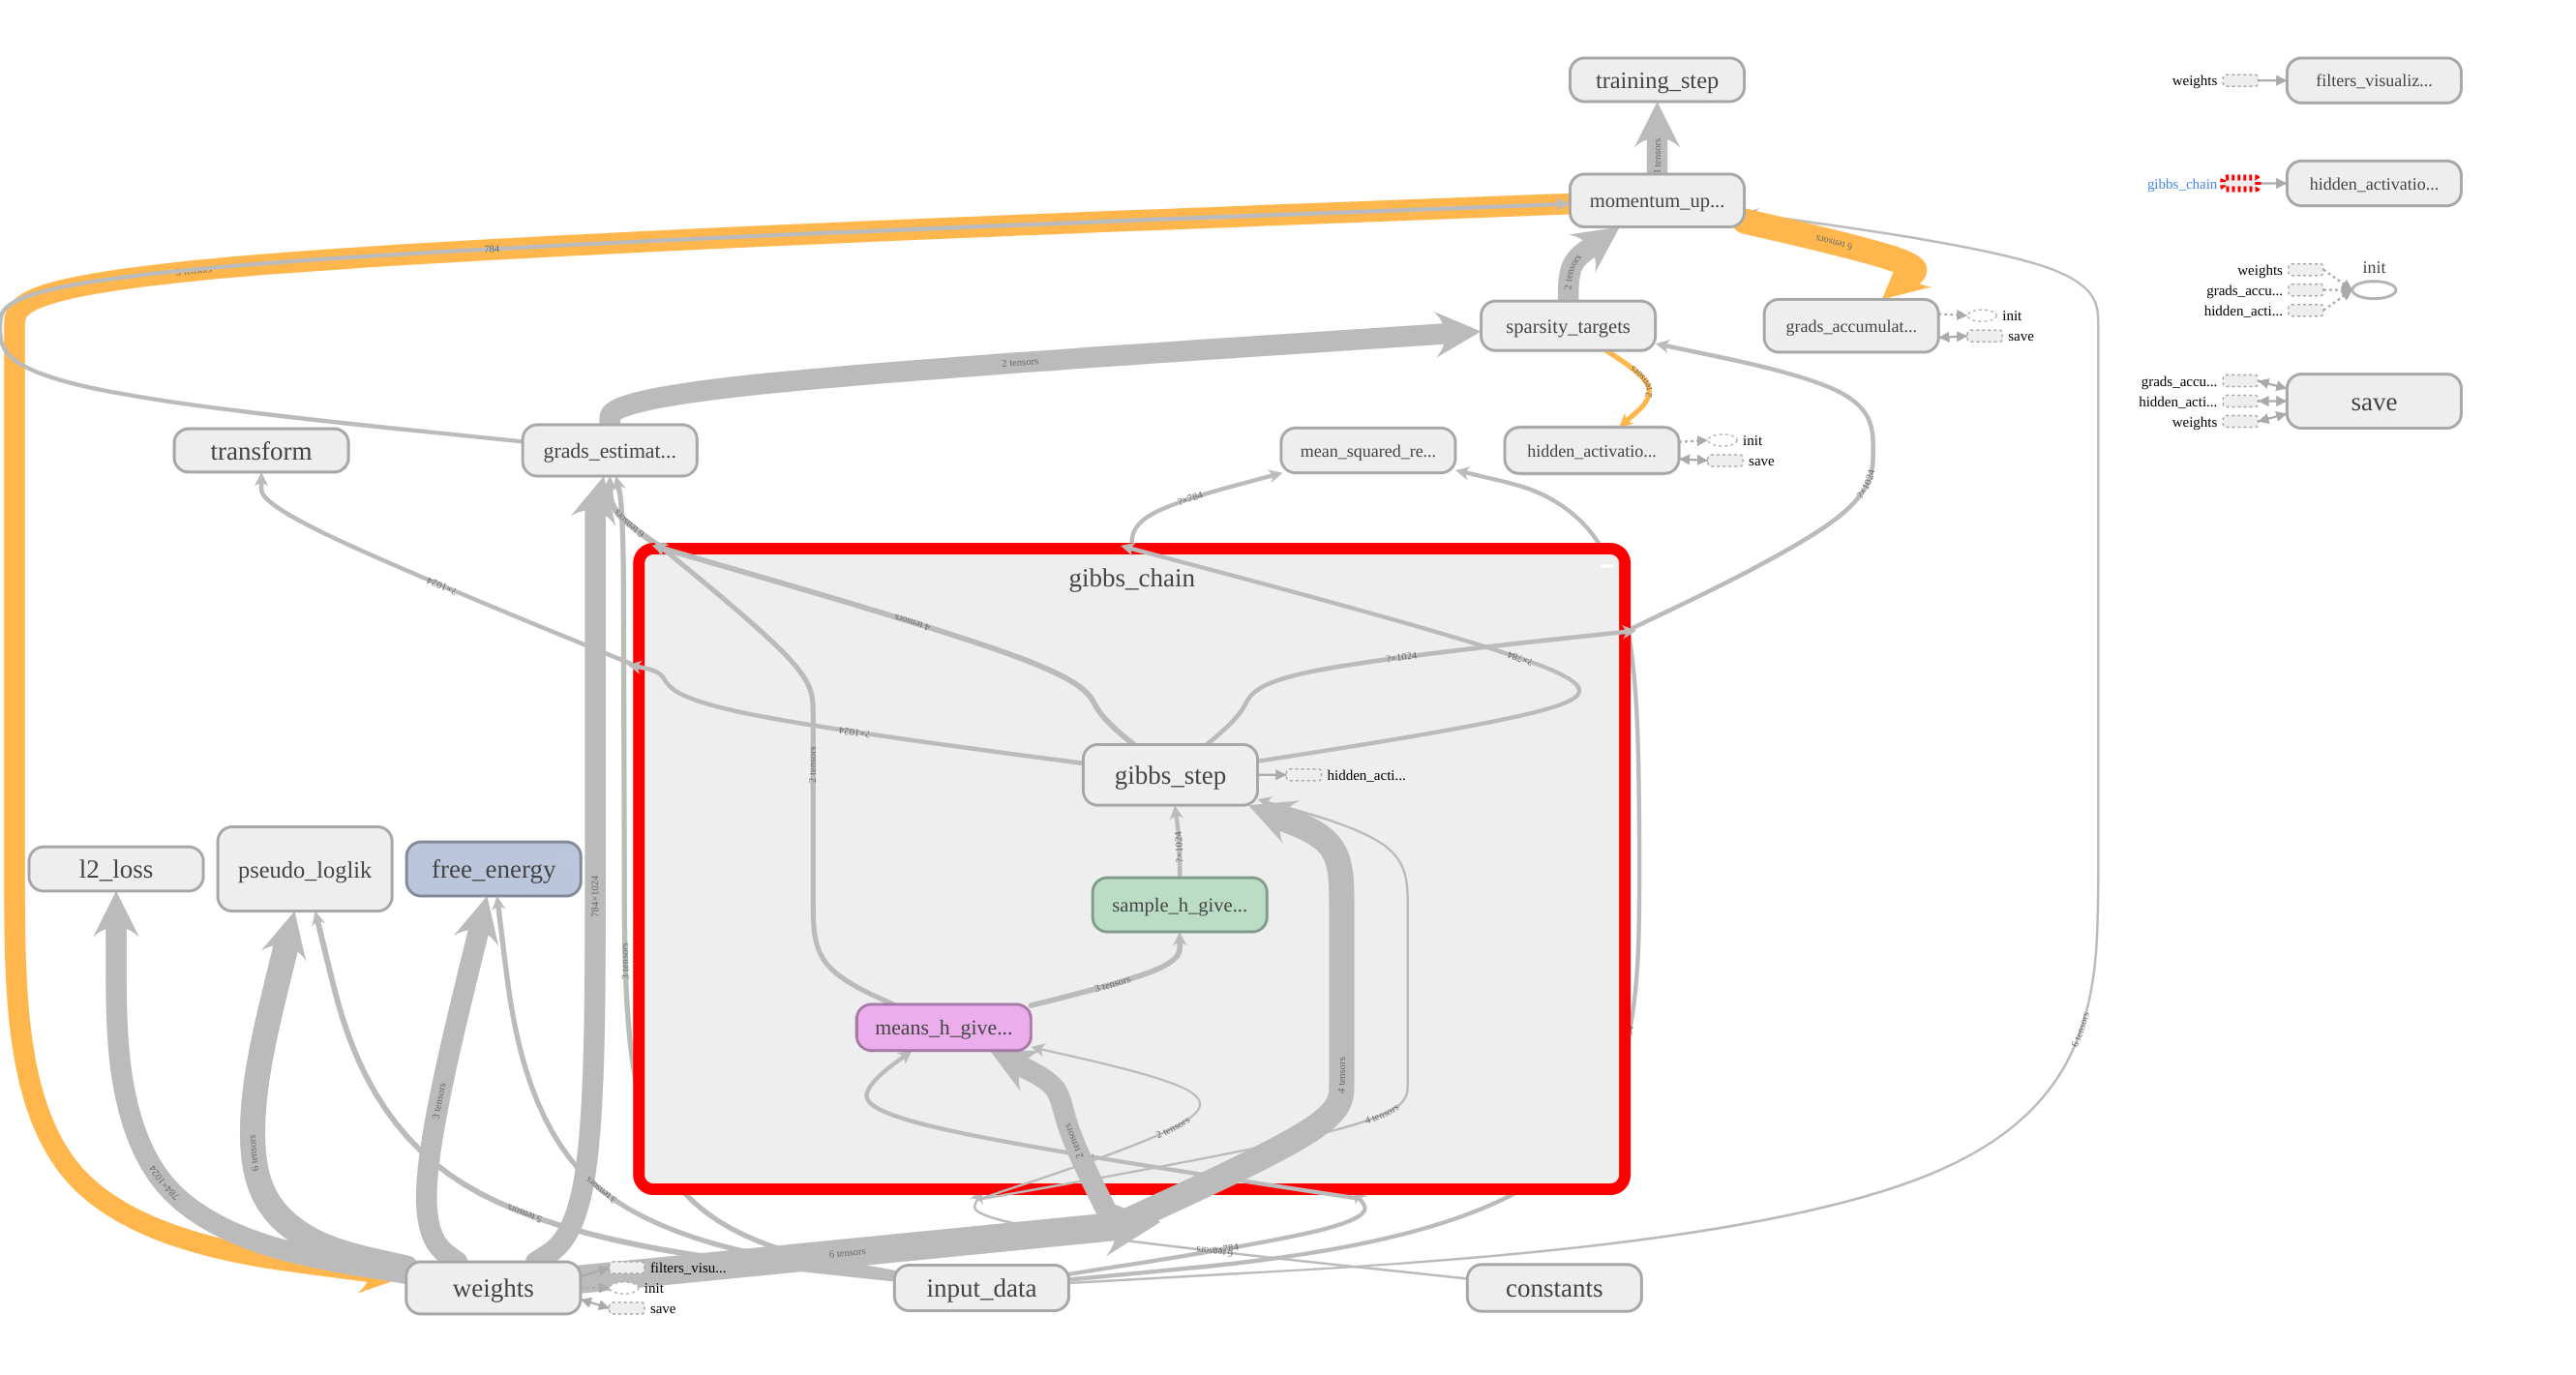
\includegraphics[width=5.6in]{rbm/tf_graph.png}
\caption{\emph{Top}: When single precision is used, the difference in performance is negligible compared to the double precision, training however is almost 2.5 times faster (pseudo log-lik is slightly more noisy at the beginning of training though). \emph{Bottom}: high-level computational graph for RBM.}
\end{mdframed}
\end{figure}

\clearpage
